%%%%%%%%%%%%%%%%%%%%%%%%%%%%%%%%%%%%%%%%%%%%%%%%%%%%%%%%%%%%%%%%%%%%%%%%%%%%
% AGUJournalTemplate.tex: this template file is for articles formatted with LaTeX
%
% This file includes commands and instructions
% given in the order necessary to produce a final output that will
% satisfy AGU requirements, including customized APA reference formatting.
%
% You may copy this file and give it your
% article name, and enter your text.
%
%
% Step 1: Set the \documentclass
%
%

%% To submit your paper:
\documentclass[draft]{agujournal2019}
\usepackage{url} %this package should fix any errors with URLs in refs.
\usepackage{lineno}
\usepackage[inline]{trackchanges} %for better track changes. finalnew option will compile document with changes incorporated.
\usepackage{soul}
\usepackage{amsmath}
\usepackage{siunitx}
\usepackage{color}
\newcommand{\red}[1]{\textcolor{red}{#1}}
\newcommand{\blue}[1]{\textcolor{blue}{#1}}

\linenumbers
%%%%%%%
% As of 2018 we recommend use of the TrackChanges package to mark revisions.
% The trackchanges package adds five new LaTeX commands:
%
%  \note[editor]{The note}
%  \annote[editor]{Text to annotate}{The note}
%  \add[editor]{Text to add}
%  \remove[editor]{Text to remove}
%  \change[editor]{Text to remove}{Text to add}
%
% complete documentation is here: http://trackchanges.sourceforge.net/
%%%%%%%

\draftfalse

%% Enter journal name below.
%% Choose from this list of Journals:
%
% JGR: Atmospheres
% JGR: Biogeosciences
% JGR: Earth Surface
% JGR: Oceans
% JGR: Planets
% JGR: Solid Earth
% JGR: Space Physics
% Global Biogeochemical Cycles
% Geophysical Research Letters
% Paleoceanography and Paleoclimatology
% Radio Science
% Reviews of Geophysics
% Tectonics
% Space Weather
% Water Resources Research
% Geochemistry, Geophysics, Geosystems
% Journal of Advances in Modeling Earth Systems (JAMES)
% Earth's Future
% Earth and Space Science
% Geohealth
%
% ie, \journalname{Water Resources Research}

\journalname{JGR: Oceans}


\begin{document}

%% ------------------------------------------------------------------------ %%
%  Title
%
% (A title should be specific, informative, and brief. Use
% abbreviations only if they are defined in the abstract. Titles that
% start with general keywords then specific terms are optimized in
% searches)
%
%% ------------------------------------------------------------------------ %%



\title{=enter title here=}

%% ------------------------------------------------------------------------ %%
%
%  AUTHORS AND AFFILIATIONS
%
%% ------------------------------------------------------------------------ %%

% Authors are individuals who have significantly contributed to the
% research and preparation of the article. Group authors are allowed, if
% each author in the group is separately identified in an appendix.)

% List authors by first name or initial followed by last name and
% separated by commas. Use \affil{} to number affiliations, and
% \thanks{} for author notes.
% Additional author notes should be indicated with \thanks{} (for
% example, for current addresses).

% Example: \authors{A. B. Author\affil{1}\thanks{Current address, Antartica}, B. C. Author\affil{2,3}, and D. E.
% Author\affil{3,4}\thanks{Also funded by Monsanto.}}

\authors{=list all authors here=}


% \affiliation{1}{First Affiliation}
% \affiliation{2}{Second Affiliation}
% \affiliation{3}{Third Affiliation}
% \affiliation{4}{Fourth Affiliation}

\affiliation{=number=}{=Affiliation Address=}
%(repeat as many times as is necessary)

%% Corresponding Author:
% Corresponding author mailing address and e-mail address:

% (include name and email addresses of the corresponding author.  More
% than one corresponding author is allowed in this LaTeX file and for
% publication; but only one corresponding author is allowed in our
% editorial system.)

% Example: \correspondingauthor{First and Last Name}{email@address.edu}

\correspondingauthor{=name=}{=email address=}

%% Keypoints, final entry on title page.

%  List up to three key points (at least one is required)
%  Key Points summarize the main points and conclusions of the article
%  Each must be 100 characters or less with no special characters or punctuation and must be complete sentences

% Example:
% \begin{keypoints}
% \item	List up to three key points (at least one is required)
% \item	Key Points summarize the main points and conclusions of the article
% \item	Each must be 100 characters or less with no special characters or punctuation and must be complete sentences
% \end{keypoints}

%\begin{keypoints}
%\item 
%\item
%\item  
%\end{keypoints}

%% ------------------------------------------------------------------------ %%
%
%  ABSTRACT and PLAIN LANGUAGE SUMMARY
%
% A good Abstract will begin with a short description of the problem
% being addressed, briefly describe the new data or analyses, then
% briefly states the main conclusion(s) and how they are supported and
% uncertainties.

% The Plain Language Summary should be written for a broad audience,
% including journalists and the science-interested public, that will not have 
% a background in your field.
%
% A Plain Language Summary is required in GRL, JGR: Planets, JGR: Biogeosciences,
% JGR: Oceans, G-Cubed, Reviews of Geophysics, and JAMES.
% see http://sharingscience.agu.org/creating-plain-language-summary/)
%
%% ------------------------------------------------------------------------ %%
\newcommand{\mpryr}{~m~yr\textsuperscript{-1}}


%% \begin{abstract} starts the second page

\begin{abstract}
[ enter your Abstract here ]
\end{abstract}

\section*{Plain Language Summary}
[ enter your Plain Language Summary here or delete this section]


%% ------------------------------------------------------------------------ %%
%
%  TEXT
%
%% ------------------------------------------------------------------------ %%
\section{Introduction}\label{S:Introduction}
%we have seen big changes, and they're mostly driven by increased basal melting

Ice sheets and ice shelves in the Amundsen sea sector of Antarctica have undergone significant changes in recent years characterized by an increasing rate of ice loss~\cite{Paolo2015Science}, grounding line retreat and glacier acceleration. These changes have been particularly prominent for Pine Island Ice Sheet in the eastern Amundsen Sea, which experienced a 70\% increase in ice flux and close to doubling of surface velocity between 1974 and 2013~\cite{Mouginot2014GRL}, while its grounding line retreated some 31~km at its centre between 1992 and 2011~\cite{Rignot2014GRL}. Increased basal melting has been implicated as a key driver of these changes~\cite{Pritchard2012Nature}: backstresses (or buttressing forces) that originate from contact with ice rumples or embayments, for example, are transferred to the upstream grounded ice, restraining its flow; thinning ice shelves therefore offer less buttressing to ice sheets, leading to an increase in the flux of ice from the grounded to floating regions of the ice sheet~\cite{Gudmundsson2013Cryo, Gudmundsson2019GRL,Gagliardini2010GRL,Goldberg2019GRL}.

%depth of the pycnocline is the most important factor
The main source of heat for ice shelf melting in the Amundsen Sea sector of Antarctica is Circumpolar Deep Water (CDW), which sits below (it is more dense than) lighter Winter Water. In the Amundsen Sea, the pycncocline that separates the two water masses remains mostly above the level of the continental shelf break~\cite{Heywood2016Oceanography}, allowing a significant amount of heat to reach ice shelves. The depth of the pycnocline is not constant, but varies significantly on decadal timescales~\cite{Jenkins2018NatureGeo}. 

%ridge in PIG makes pycnocline picture more complicated
For Pine Island, this simple `pycnocline depth' picture is complicated by the presence of a seabed ridge located several tens of kilometers upstream of the grounding line, which protrudes several hundred metres above the seabed (figure~\ref{fig:figure1}). This ridge, in combination with the presence of the ice shelf above it, acts as a topographic barrier which restricts the access of CDW to an inner cavity that has formed between the ridge and the grounding line since the ice shelf likely retreated from this ridge in the late 1940s~\cite{Jenkins2010NatureGeo, DeRydt2014JGeophysResOceans, DeRydt2016JGeophysResEarthSurf}. The particular geometry of the cavity means that the strength of the barrier is strong dependent on the pycncoline depth: at its shallowest, the pycnocline sits above the depth of the ridge crest, and a large amount of modified CDW is able to spill into the inner cavity~\citep{Dutrieux2014Science}; in contrast, at its lowest, the pycnocline sits someway below the ridge crest and CDW access is severely restricted.  As a result, melting of Pine Island Glacier has a strong sensitivity to hydrographic conditions in Pine Island Bay: Dutrieux et al. reported that the total freshwater flux from the fast flowing part of Pine Island Glacier in 2009 (80~km\textsuperscript{3}~year\textsuperscript{-1}), when the pycnocline was at its second highest level on record, was more than double its value in 2012 (37~km\textsuperscript{3}~year\textsuperscript{-1}), when the pyncocline was at the second lowest recorded depth.

%another thing we have seen is significant calving events
In addition to it's unique geometric controls on melting, the recent calving of Pine Island Ice Shelf also stands out amongst Amundsen Sea terminating shelves. While calving events are a typical part of the life cycle of an ice shelf -- calving and melt contribute similarly to the ice sheet mass losses~\cite{Rignot2013Science}, which must balance the upstream accumulation experienced upstream inf a glacier is in equilibrium -- the recent retreat of the PIIS front suggests that the calving rate is far higher than would be required to maintain an equilibium; the ice front retreated approximately 26km between 2009 to 2020 (figure~\ref{fig:figure1}), with the majority of this retreat happening over 2015--2020~\cite{Lhermitte2020PNAS, Joughin2021ScienceAdv}. These changes correspond to a more-than-doubling of the calving rate, from approximately 4~km~year\textsuperscript{-1} to approximately 9~km~year\textsuperscript{-1}.

%at present, the ridge is located approx x km downstream of the ridge crest. The changes some far have been implicated in a speed up because of a loss of buttressing, but might the changes have also led to a relaxation of the topographic barrier and thus and increase in melt rates (that would only be evidenced on longer timescales(?)) [key question one]
As of 2020, the ice front is located approximately 20~km downstream of the ridge: the ice front is now closer to the ridge crest that the location of the ice front before 2015. The loss of buttressing associated with this retreat has been shown to be responsible for the significant speed up of PIG since 2015~\cite{Joughin2021ScienceAdv}. However, given that the topographic barrier to CDW relies on the combination of ice draft \textit{and} seabed ridge, the recent calving events begs the following question about future: have recent calving events relaxed the topographic barrier, leading to significant changes in melting in PIIS?

%but also, in future, we might have further calving events because or preconditioning and or MICI that might bring to ridge to the crest. How might these potential future calving events lead to changes in melt rates? [key question two]
Here, in addition to addressing the effect on melt rates of calving events that have already happened, we also consider changes that result from potential future calving events. Indeed, it has been suggested that damage to the ice shelf has preconditioned PIIS to further signifcant calving events~\cite{Lhermitte2020PNAS} and that if calving presents a higher ice cliff to the ocean, that may trigger runaway calving events (the so called marine ice cliff instability~\cite{DeConto2016Nature}). Both of these mechanisms may lead to significant calving in the future; the second main question we aim to answer in this paper is: how might these potential future calving events lead to changes in melt rates?

In this paper, we use a combination of idealized and realistic simulations to assess how, and why, melt rates in PIIS will respond to past and potential future calving events. We begin in \S\ref{S:Experiment} with a description of the idealized experiments, including setting out details of the ocean model used, and the various cavity geometries, and hydrographic forcings that change between experiments. We perform nine idealized experiments in total, and one of these is selected as a baseline; in \S\ref{S:Baseline} we discuss how and why the melt rate responds to calving for the baseline experiments. In the following two sections, we discuss how the picture presented in \S\ref{S:Baseline} changes for different cavity geometries (\S\ref{S:Results:H}) and hydrographic forcings (\S~\ref{S:Results:P}). In \S\ref{S:Realistic}, we describe an analogous experiment using a geometry that closely matches real world conditions for PIIS. Guided by the results of the idealized experiments, we assess the response of melt rates to calving events. Finally, in \S\ref{S:Discussion}, we discuss the implications of our results and provide concluding remarks.

%what we're going to do: use a combination of idealized and real world modelling to attempt to answer these questions. 

%in this paper, we explore the response of melting to calving in an idealized setup. We aim to isolate the physical processes responsible. Idealized modelling also means that 
%In this paper, we aim to 



%\begin{figure}
%    \centering
%    \includegraphics{}
%    \caption{Info on realistic PIG}
%    \label{fig:figure1}
%\end{figure}

\section{Experiment Details}\label{S:Experiment}
\red{I think it would be good to have a table with all of the experiments in!}


%broad overview of the experiemnts
We perform a total of nine experiments, each corresponding to a unique pair of parameters that characterize the hydrographic forcing, the strength of the barrier provided by the shelf, which are known to be variable in practice (section 1). Within each experiment, we perform ten simulations in which the ocean circulation is resolved explicitly using the MIT general circulation model (MITgcm): the first `default' (or `uncalved') simulation  corresponds to a configuration that captures the essential features of the Pine Island Cavity in 2009, while in the nine further `calving' simulations, sections of the ice shelf in the default run are removed subsequently, thus simulating the effect of calving (we use the word calving henceforth as a proxy for this description). Other than removing sections within each experiment, the ice shelf geometry does not change within each experiment (but may change between experiments, see section \ref{S:Experiment:Geometry}). Ice shelves therefore enter passively, via the exchange of heat and salt at the ice-ocean interface alone; a passive description of ice shelves (i.e. not including any ice sheet or ice shelf dynamics) is sufficient for this study since we are primarily interested in response of melt rates to ice shelf calving, which occur on timescales much shorter than on which the ice responds dynamically to perturbations in melting. In the following sections we provide further details of the ocean model and experimental setup, including the motivation for various parameter choices.
\begin{figure}
    \centering
    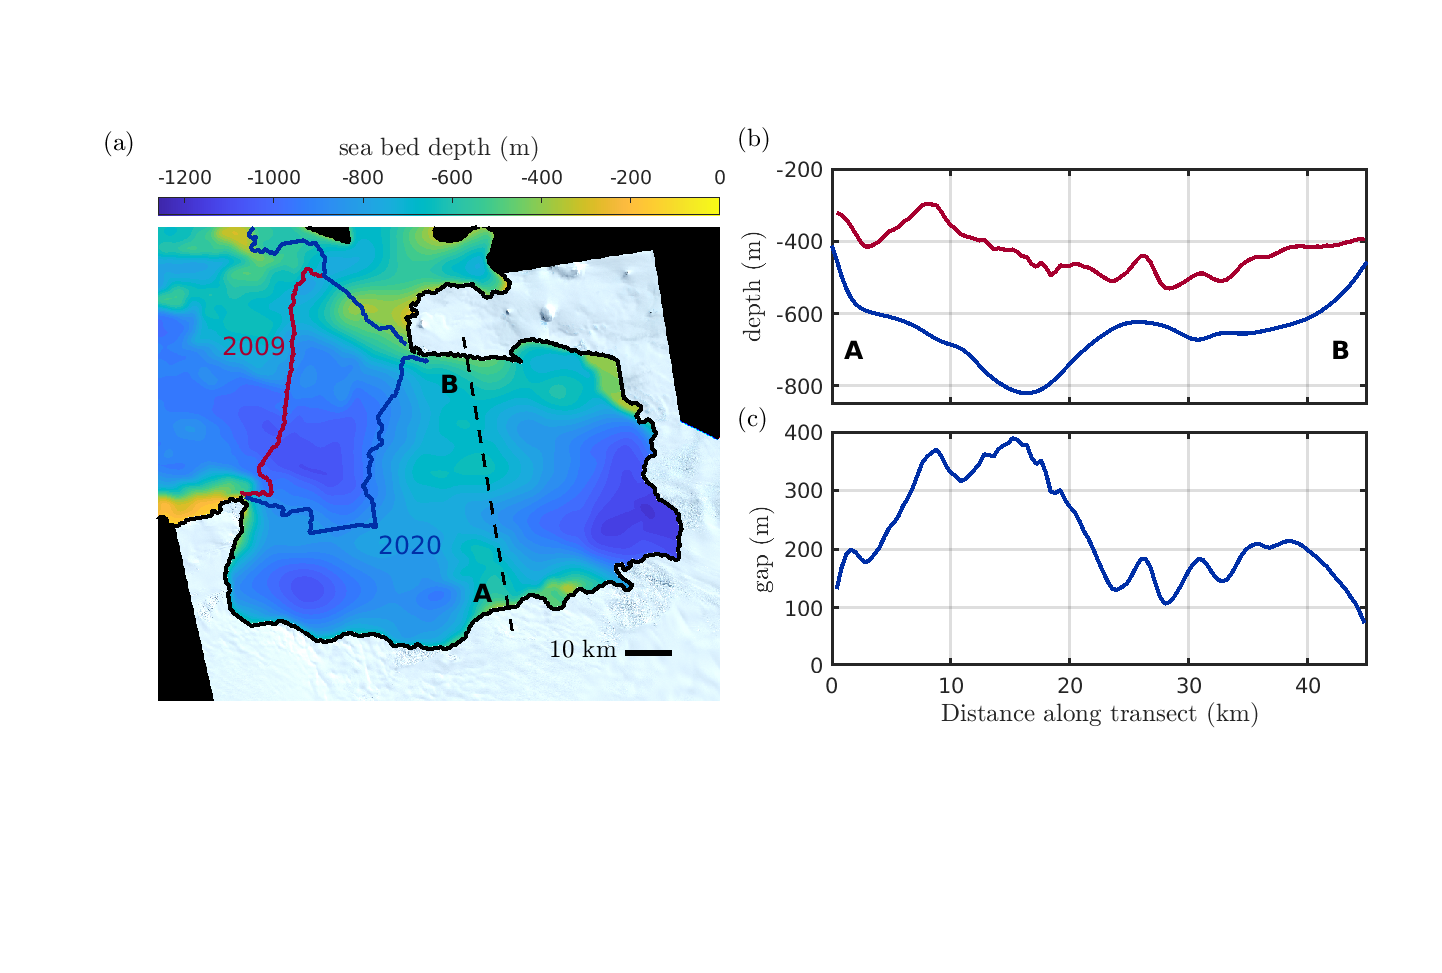
\includegraphics[width = \textwidth]{../make_figures/plots/figure1.eps}
    \caption{figure 1: (a) PIG bathymetry with (b) bathymetry and ice topo along contour, (c) gap. \red{Need to add (a), (b), (c) labels and crop whitespace. Also add co-ordinate lines?}}
    \label{fig:figure1}
\end{figure}
\begin{figure}
    \centering
    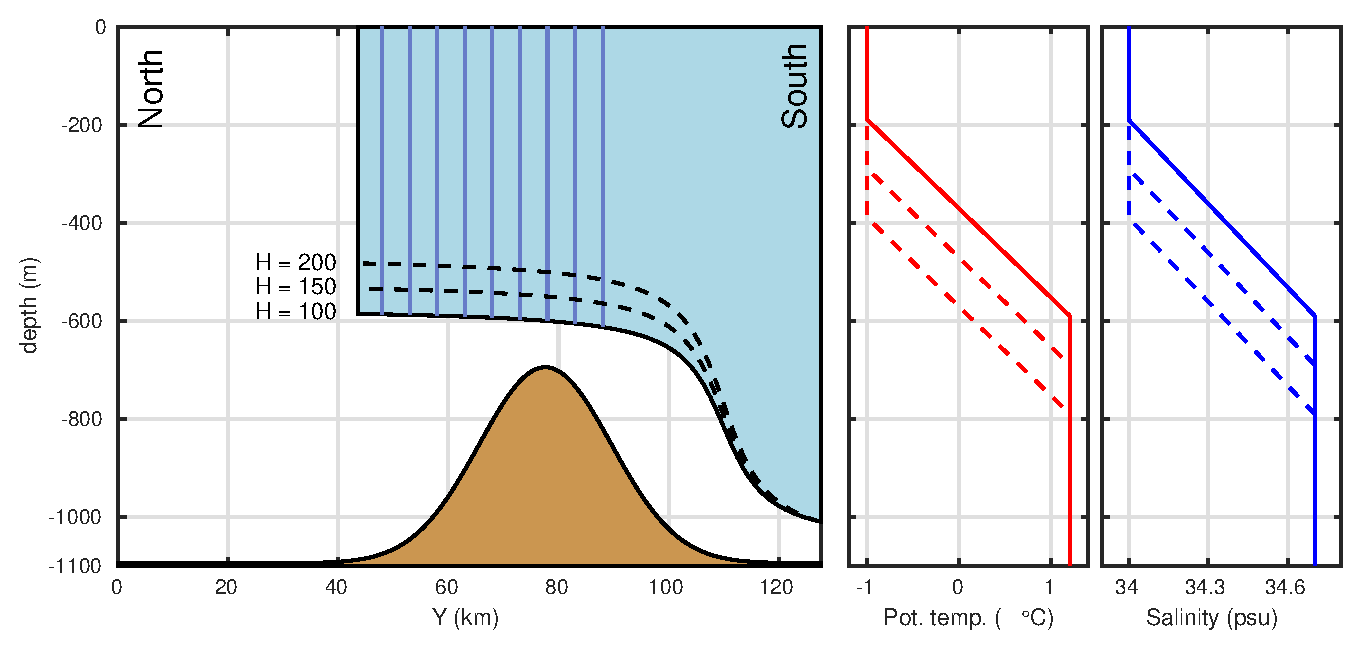
\includegraphics[width = \textwidth]{../make_figures/plots/figure2.eps}
    \caption{(a) Schematic diagram of the experimental setup. The ocean domain consists of the gridded area, which is bordered by a passive ice shelf (shaded blue) and seabed ridge a (shaded brown). Solid and dashed black lines indicate the ice shelf geometry used in the default simulation for the three values of the ridge-gap parameter $H$=100~m, $H$=150~m, and $H$=200~m, as labelled. Solid blue lines indicate the ice front in the calving experiments, which are located 80, 75, 70, 65, 60, 55, 50, 45, and 40~km north of the southern end of the domain. The shaded red region indicates the inner cavity (see main text), defined as those locations in the ocean domain that are within 30~km of the southern end of the domain. (b) Salinity and temperature profiles used in the experiments (red and blue curves), with $P$ = 600~m (solid), $P$ = 700~m (dashed), $P$ = 800~m (dot-dashed) as indicated by the label. Grey lines correspond to temperature and salinity profiles taken from CTD measurements in Pine Island Bay during the austral summers of 2009 (light grey) and 2012 (dark grey).  \red{Possibly add restoring region?}}
    \label{fig:figure2}
\end{figure}

\subsection{Details of Ocean Model}\label{S:Experiment:Model}
The MITgcm is a z-level general circulation model that includes a partial-cell treatment of topography, allowing an accurate description of both the seabed and ice draft. Our model grid consists of 110 layers with a vertical spacing of 10~m, and a horizontal resolution of 400m. We use the MITgcm in hydrostatic mode with a implicit nonlinear free surface scheme, a third-order direct space-time flux limited advection scheme, a non-linear equation of state~\citeA{Mcdougall2003JAtmosOceanTech}, and the Pacanowski-Philander~\cite{Pacanowski1981JPhysOcean} scheme parametrizes vertical mixing. Constant values of 15 and 2.5~m\textsuperscript{2}~s\textsuperscript{-1} are used for the horizontal Laplacian viscosity and horizontal diffusivity. The equations are solved on an $f$-plane with $f = -1.4\times10^{-4}~\text{s}^{-1}$.

Each simulation is ran for a total of 12 months, using a timestep of 30~\si{seconds}, after which time the configuration reaches a steady state. The melt rates reach approximately 95\% of their final values with three months \red{(see Appendix?)}. All results presented here are averaged over months nine to twelve in the simulation. 

The MITgcm includes a static representation of ice shelves~\cite{Losch2008JGeophysResOceans}. Ice shelf melting is implemented using the so-called "three-equation formulation"~\cite{Holland1999JPhysOcean} that describes the exchange of heat and salt across the ice-ocean boundary. The implementation of this scheme in MITgcm has been described in detail elsewhere~\cite[for example]{DeRydt2014JGeophysResOceans,Dansereau2014JGROceans} but we note that thermal exchange across the ice-ocean interface is typically dominated by latent heat (a consequence of the fact that temperatures difference between ice shelves and the adjacent boundary layer is on the order of several degrees Celsius, while the characteristic temperature associated with latent heat removal is -84 degrees Celsius). With latent heat dominate thermal exchange, the three equation formulation gives the melt rate $\dot{m}$ as
\begin{equation}\label{E:MeltRate}
    \dot{m} = \frac{c_p \gamma_T (T - T_b)}{L}.
\end{equation}
Here $c_p = 3947~\si{\joule \kilogram}^{-1}$ is the specific heat capacity of water, $T$ is the temperature of the ambient ocean, $T_b$ is the temperature at the ice shelf base, which must be at the local freezing point, and $\gamma_T$ is a heat exchange co-efficient. The heat exchange coefficient has an approximately linear relationship on $u^*$, the ocean speed adjacent to the ice shelf base~\cite{Holland1999JPhysOcean}; assuming a perfectly linear relationship, equation~\eqref{E:MeltRateUdT} yields
\begin{equation}\label{E:MeltRateUdT}
    \dot{m} \propto u^* (T - T_b).
\end{equation}
We shall return to~\eqref{E:MeltRateUdT} when diagnosing the reasons for changes in the melt rate as the ice shelf calves.

All parameter values used in the three equation formulation here are as in~\citeA{Holland1999JPhysOcean}, with the exception of the drag co-efficient, which is set to $4.5\times10^{-3}$, a value is more appropriate for Pine Island Glacier~\cite{Dutrieux2014Science} (the drag coefficient that enters in the momentum balance, which can be set independently, remains at the default value of $2.5\times 10^{-3}$).

\subsection{Ice Shelf Geometry and Seabed Bathymetry}\label{S:Experiment:Geometry}
Our idealized setup is shown schematically in figure~\ref{fig:figure2}a: it is uniform in the zonal direction, along which the $x$-axis is aligned, and the $y$-axis is aligned along the meridional direction (although PIG is aligned approximately East-West, we assume here that it is aligned East-West, as is standard~\cite{Grosfeld1997JGROceans, DeRydt2014JGeophysResOceans}).

The sea bed has a Gaussian profile,
\begin{equation}\label{E:Experiment:Bed}
    b(x,y) = -1100 + 400 \exp\left[-\frac{\left(y - 50\times 10^3\right)^2}{2\sigma^2}\right],
\end{equation}
where $\sigma = 12$~km is the length scale over which this profile decays towards zero. The profile~\eqref{E:Experiment:Bed} corresponds to a ridge that peaks 50km from the southern end of the domain, which can be considered as the grounding line, at a height of 400m (note that the cavity thickness is prevented from reaching zero at the grounding line as the MITgcm requires at least two grid cells in the vertical to permit horizontal transfer). 

The variability in both Pine Island Ice Shelf draft and the height of the seabed ridge result in a ridge-draft gap that varies between approximately 100m at its narrowest to greater than 300m at it's widest (figure~\ref{fig:figure1}). Since we assumed a constant sea bed geometry, we aim to capture the effect of variability in the ridge-draft gap by considering different values of $H$, the vertical distance between the crest of the seabed ridge and the ice shelf base; $H$ enters only the model only via the ice profile, which, following~\citeA{DeRydt2014JGeophysResOceans}, takes the form
\begin{equation}
    h(y) = \begin{cases}
    \left(\frac{310 + H}{2.64}\right)\tan^{-1}\left(\frac{y}{5882} -3\right) & \text{for}~y < y_f,\\
    0  & \text{for}~y \geq y_f.
    \end{cases}
\end{equation}
Here $y_c$ is the location of the ice front, which is varied in order to simulate calving (see below). We stress that these ice profiles are not obtained from ice dynamics considerations, but do feature a flatter section beyond the ridge and a steeper section inside the ridge that is observed in practice (figure~\ref{fig:figure2}a).

We use three different values of $H$: $H$=100~m, $H$=150~m, and $H$=200m. The smallest value, $H = 100$m, corresponds to the minimum gap between the ice shelf and ridge that is observed in Pine Island (figure~\ref{fig:figure1}), while the largest value, $H$=200m, corresponds to an upper bound, beyond which the melt response to calving is negligible, as we shall see. The third value, $H$=150~m is an intermediate value between $H$ at which the melt rate is highly sensitive and weakly sensitive to calving.

Within each experiment, the vary the front position $y_f$ is systematically reduced by removing sections of ice, to simulate calving. The ten simulations within each experiment use values $y_f$ = 84 (default), 80, 75, 70, 65, 60, 55, 50, 45, and 40~km, which correspond to calved lengths of $l_c$= 0, 4, 9, 14, 19, 24, 29, 34, 39, and 44~km, respectively. There are both pragmatic and physical reasons for this choosing this particular range: the default experiment with $y_f$= 84~km corresponds to the distance of the ice front in PIG in 2009, before significant calving took place in the late 2010s; the lowest value, $y_f$ = 40~km, is chosen as a compromise between a configuration in which the ice front has calved a significant distance beyond the ridge, which retains a significant area that is shared by each experiment: as we discuss further in \S\ref{S:Baseline}, the area over which melt rates are averaged should be invariant to calving for a rigorous assessment of changes with calving. The computational expense of ocean simulations together with a large number of experiments means that the number of simulations within the range is restricted to ten.

\subsection{Hydrographic Forcing}\label{S:Experiment:Hydrography}

As discussed in \S\ref{S:Introduction}, the presence of a seabed ridge in Pine Island Glacier means that melt rates are particularly sensitive to the ocean state in the far away from the cavity (the hydrographic forcing); we therefore expect that the melting response to calving will also have a sensitive dependence on hydrographic forcing. To assess this sensitivity, we repeat each of the experiments with different values of the ridge-gap parameter $H$ described in the previous section with three different hydrographic forcings, which are imposed on the model by means of a restoring boundary condition at the northern end of the domain (figure~\ref{fig:figure2}): at this boundary, the temperature and salinity are restored to specified vertical profiles over a distance of five horizontal grid cells (total length 2km) with a restoring timescale that varies from 12~h at the boundary to 60~h at the interior of this restoring regions. (The model includes solid walls with a free slip condition at the southern, western, and eastern sides of the domain.)

%what do our profiles look like
The three temperature and salinity profiles to which the ocean is restored are shown schematically in figure~\ref{fig:figure2}b,c. Both the temperature and salinity profiles are piecewise linear, with constant conditions in both a lower layer (temperature $1.2~\si{\celcius}$, salinity $34.7$~psu) and upper layer (temperature $-1~\si{\celcius}$, salinity $34$~psu) separated by a pycnocline of thickness 400~m. The pycnocline begins at a variable depth $P$ (a higher $P$ corresponds to a deeper pycnocline), which parametrizes the whole profile; our three hydrographic forcings use $P = 600$, $700$, and $800$. 

%why do we choose these conditions
These piecewise linear profiles correspond to (simplified versions of) typical conditions for the Pine Island Bay~\cite{Jacobs1996GRL, Dutrieux2014Science, Jenkins2018NatureGeo} (see figure~\ref{fig:figure2}a,b). The upper and lower layers are dominated by Winter Water and Modified Circumpolar Deep Water, respectively. A record of hydrographic conditions in the Amundsen Sea indicates significant variability in the depth of the pycnocline varies considerably on interannual timescales~\cite{Dutrieux2014Science}; the profiles with $P = 600$ and $P = 800$ correspond to the years 2009 and 2012, respectively, which span the range of observed conditions: in 2012, the average depth of the pycnocline was at the lowest on record, while in 2009, the average depth of the pycnocline was at the highest on record. 

%wrap up the experiments:\ 
The nine experiments can be uniquely identified by a $(H,P)$ pair, where $H$ $\in \{100, 150, 200\}$ and $P$ $\in \{600, 700, 800\}$. We consider the extreme scenario with the strongest topographic barrier and warmest hydrographic forcing, $(H,P) = (100,600)$ to be the baseline; in the following section, we describe the results of this baseline experiment, before describing in sections~\ref{S:Results:H} and~\ref{S:Results:P} how this picture changes for different values of $H$ and $P$, respectively.

\section{Result for the Baseline Experiments}\label{S:Baseline}
In this section, we describe the results for the baseline experiment with $H$ = 100~m and $P$ = 600~m, which correspond to the profiles with solid lines in figures~\ref{fig:Schematic}a--c. We begin by describing the steady state configuration for the uncalved run, and then describe how, and why, calving changes the melt rate.

\subsection{Default Run: $H$=100~m, $P$=600~m}\label{S:Baseline:Default}
%describe each of what we see: melt rate, general observations
Ice-ocean properties that characterise the default simulation are shown in figure~\ref{fig:figure3}. Melt rates (figure~\ref{fig:figure3}a) are mostly below  15\mpryr everywhere, except for a region located within 20~km of the grounding line, where maximum melt rates of reach a maximum of approximately 120\mpryr. The average melt rate over the whole shelf is approximately 20\mpryr; this is lower than the observed value of 33$\pm$2 that has been observed for PIG in 2009 (to which the $P=600$ case corresponds), as is to be expected given that the configuration in this simulation has the tightest topographic control on warm water inflow that is observed for PIG applied everywhere.

%introduce the idea of the inner cavity, why do we use this metric
It is useful to introduce the `inner cavity': the area of the ocean that is located within 30~km of the Southern end of the domain (indicated by the red shaded region in figure~\ref{fig:figure2}a). We use the mean melt rate in the inner cavity (solid red line figure~\ref{fig:figure2}a) as our metric to quantify changes in melt rate with calving, and refer to this quantity henceforth as the `inner cavity melt rate'. A spatially invariant area over which the melt rate is integrated is necessary because the melt rate under the ice shelf is highly spatially variable (figure~\ref{fig:figure3}a); for example, if we removed sections of ice in the default run \textit{without} changing the melt rate pattern, those runs with less ice (i.e. significant calving) would display larger mean melt rates over the whole shelf because the highest melt rates are concentrated near the grounding line. The 30~km length of the inner cavity region reflects a compromise between permitting calving a distance beyond the ridge, while including a reasonably large section of the ice shelf over which the melt rate is averaged. In addition, this region includes the `grounding line', where changes in melting are particularly important to the dynamics of the ice sheet~\cite{Seroussi2014Cryo, Athern2017GRL}. Although the values of inner cavity melt rate are dependent on the choice of cavity, we verified that the trends and key results of the following sections are independent of the choice of inner cavity, provided that it is taken sufficiently far from the maximal extent of any of the simulations; for the choice of 30~km, the inner cavity melt rate in the default run is 46\mpryr.

%why does the melt rate look like it does
Melt rates depend strongly on the cavity circulation and thermal driving (equation~\eqref{E:MeltRate}). Cavity circulation (figure~\ref{fig:figure3}a,c) is charaterized by a cyclonic circulation which is Coriolis-driven. This circulation is directed northward and southward at the Eastern and Western boundaries ($x=$0~km and $x=$48~km), respectively. In the inner cavity, South of $y = 30$~km, the circulation is vigorous, but high melt rates are confined to within $y$ = 20~km: North of approximately $y$=20~km, a cold, fresh, and thus buoyant, meltwater plume  is adjacent to the ice-ocean interface (figure~\ref{fig:figure3}e), rather than the modified warm water that is adjacent to the ice-ocean interface for $y < $ 20~km  (figure~\ref{fig:figure3}d); the thermal driving, and thus melt rates, are significantly lower North of $y$=20~km.


%we can use the bsf 
To understand this behaviour, it is instructive to consider the barotropic stream function (figure~\ref{fig:figure3}b), which can be used to explain many of the characteristic features. If the flow is geostrophic, with buoyancy driving force balancing Coriolis forces, the barotropic flow will align with contours of constant $f/h$, where $h$ is the water column thickness and $f =$ -1.4$\times$10\textsuperscript{-4}~s\textsuperscript{-1} is the Coriolis parameter at 75${}^\circ$S; these contours correspond to lines of constant $y$, aligned East-West. There are two main potential vorticity (PV) barriers: the first is at the ice front, where the resulting divergent currents, and associated high velocities, lead to locally enhanced melt rates of up to 50\mpryr. The second is provided by the seabed ridge; as flow approaches the ridge, it is diverted Westward (figure~\ref{fig:figure2}) to retain a constant potential vorticity, and ultimately, this PV barrier is sufficiently strong that little flow is able to penetrate across the ridge (note the 0 contour at the top of the ridge in figure~\ref{fig:figure3}b). The exception to this is a strong boundary current at the East, where flow divergence and relative vorticity permit flow perpendicular to contours of constant column this thickness which is Southward (Northward) in the East (West). The result of the strong PV barrier is that a strongly topographically constrained circulation spins up inshore of the ridge, a feature that is common to more realistic simulations of Pine Island~\cite{Heimbach2012AnnGlac, Dutrieux2014Science}.

The connection between the inner and outer cavity comes exclusively via the Eastern boundary current: any warm water that might overcome the PV barrier presented by the ridge in the central trunk is blocked by the meltwater plume, which extends all the way from the ridge crest to the ice shelf base (figure~\ref{fig:figure3}e). Warm water that passes over the ridge via the boundary current is lightly modified by mixing with the meltwater plume as it does so, resulting in a bottom temperature that is slightly cooler (0.8${}^\circ$C) inshore of the ridge compared to offshore (1.3${}^\circ$C). The presence of this warm water inshore of the ridge results in enhanced melting by both providing significant heat, as well as increasing the stratification and thus strength of the topographically confined cyclonic circulation (the flow is approximately geostrophic within inshore of the ridge).

In summary, in this uncalved run with a strong topographic barrier, a topographically constrained cyclonic circulation is spun up inshore of the ridge. This circulation communicates exclusively with the outer cavity via an Eastern boundary current, which permits warm water access to the inner cavity, enhancing melting by providing both more heat and a stronger circulation. We note that despite this simulation corresponding to a topographic barrier that is expected to be stronger than reality, several features are in agreement with observations such as the presence of warm water on the inner cavity, the presence of a strong meltwater plume that is coldest inshore of the ridge, and a weak hydrographic front that forms on the Northern slope of the ridge~\cite{Jenkins2010NatureGeo}.

\begin{figure}
    \centering
    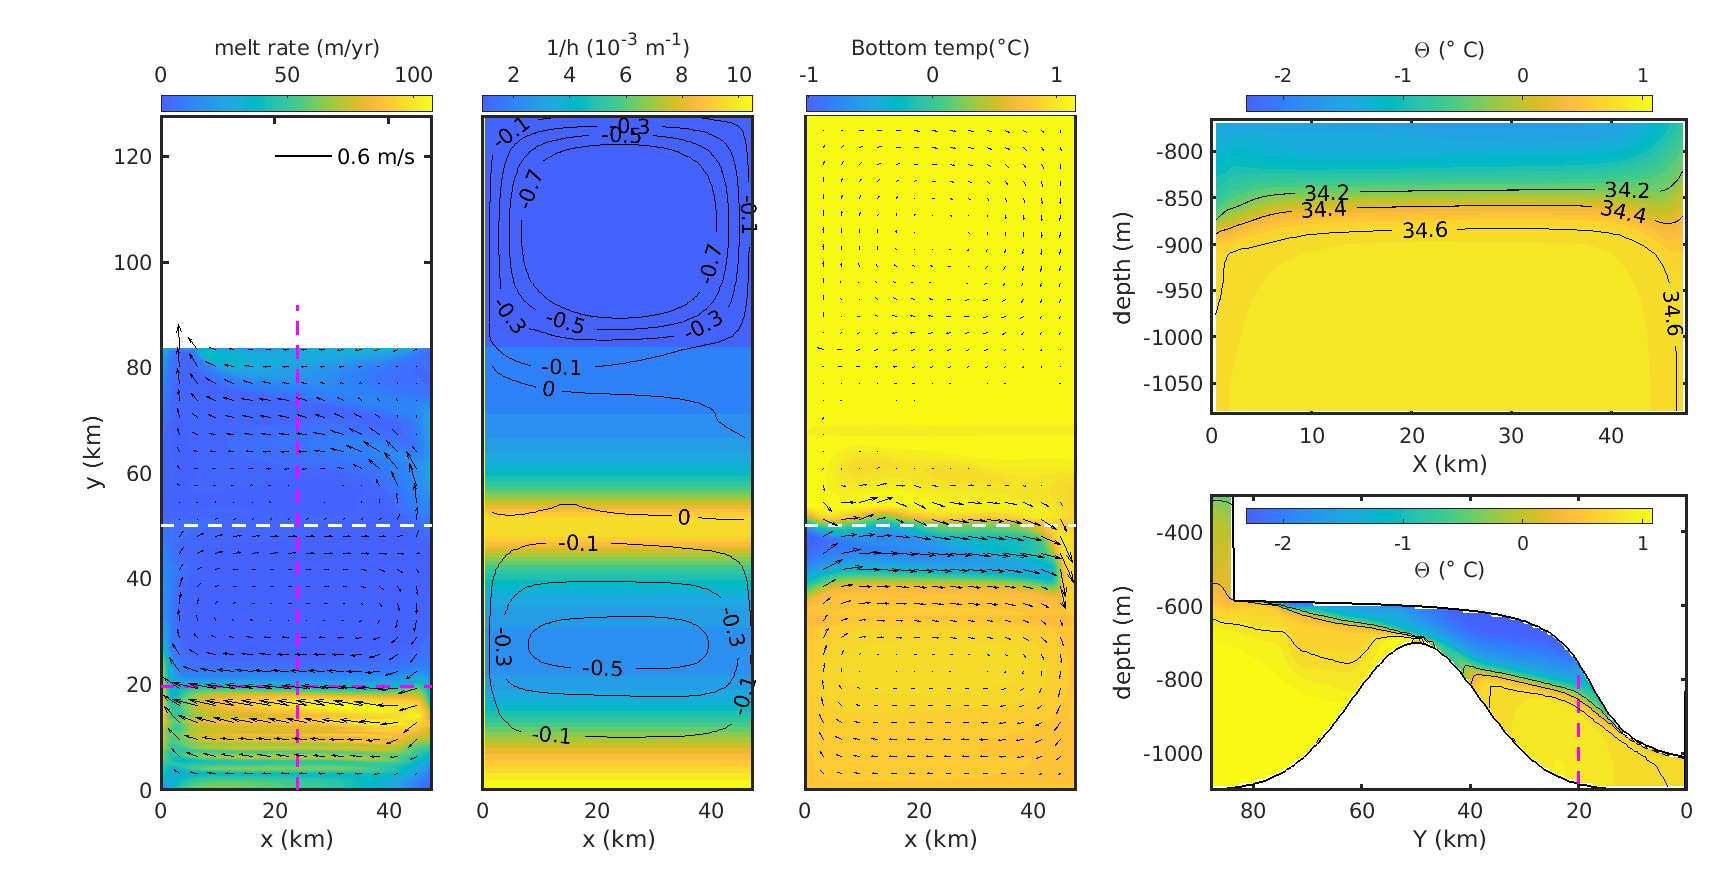
\includegraphics[width = \textwidth]{../make_figures/plots/figure3.eps}
    \caption{Ice-ocean properties that characterize the default (uncalved) run in the baseline experiment ($H$ = 100~m, $P$ = 600~m). (a) Melt rate (colours) and boundary layer velocities (arrows), averaged over the three grid cells adjacent to the ice-ocean interface. White areas correspond to open ocean. Every fifth boundary layer velocity is plotted; the black line indicates an arrow length that would correspond to 0.6~m~s\textsuperscript{-1}. The white dashed line indicates the location of the top of the ridge, while the E-W and N-S aligned dashed magenta lines indicate the location at which the cross sections in (d) and (e) are taken, respectively. (b) Inverse water column thickness $1/h$ (colours) and barotropic stream function (black contours, in units of Sv). (c) Bottom temperature (colours) and bottom current (arrows) averaged over the three grid cells closest to the ocean floor. The scale bar in (a) is also appropriate for (c). (d) Zonal cross-section taken along the E-W aligned magenta line in (a), showing potential temperature (colours) and salinity contours at the 34.2, 34.4, and 34.6~psu levels. (e) Meridional cross-section, taken along the N-S aligned magnenta line in (a), with colours and contours as in (d). The magneta dashed line indicates the location of the section correspnding to (d).}
    \label{fig:figure3}
\end{figure}

%figure 4: plots of (a) melt rate and velocity vectors, (b) geostrophic contours and BSF overlain and (c) bottom current and temperature (i.e. a la Jan 2014 paper)
\subsection{Calving Effect}
While the ice shelf front is located beyond 70~km from the grounding line, removing sections of ice increases the inner cavity melt rate only slightly (figure~\ref{fig:figure4}a). As the ice shelf front approaches the ridge, however, the melt rate increase dramatically, reaching a maximum of 73\mpryr (70\% larger than in the default run) when the ice shelf is located approximately 5~km north of the ridge crest. The following calving event, after which the ice shelf front sits immediately above the ridge, results in a significant decrease in the melt rate of approximately 15\%  (from 73\mpryr to 64\mpryr). The melt rate is then approximately independent of further calving events.


%figure 5: (a) plot of mean melt rate as a function of extent and (b) millgate decomposition 
\begin{figure}
    \centering
    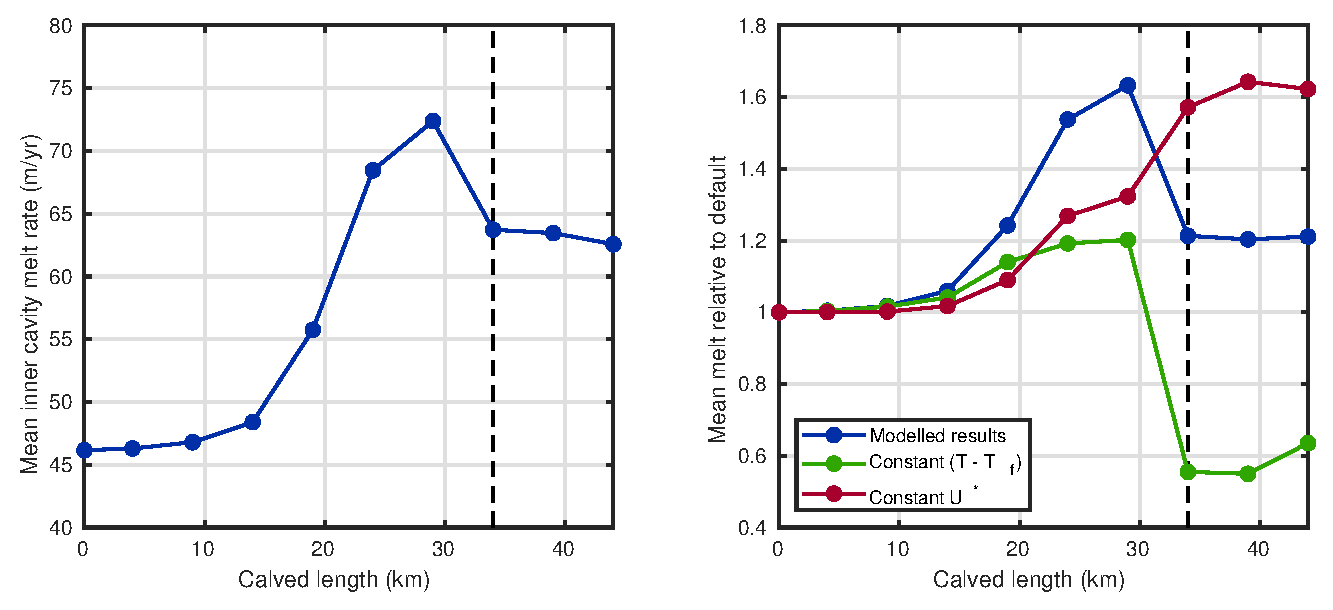
\includegraphics[width = \textwidth]{../make_figures/plots/figure4.eps}
    \caption{(a) Mean inner cavity melt rate as a function of the calved length $l_c$. The black dashed line indicates the position of the ice front when it is located directly above the seabed ridge. (b) Velocity-thermal driving decomposition: plot of the decomposition of changes in inner cavity melt rate relative to the default (uncalved) experiment (equation~\eqref{E:MillgateDecompMelt}) into changes in boundary layer speed $U_\text{effect}$ (green curve, equation~\eqref{E:MillgateDecompU}) and thermal driving $\Delta T_{\text{effect}}$ (red curve, equation~\eqref{E:MillgateDecompDT}).}
    \label{fig:figure4}
\end{figure}

%explain what the Millgate decomposition.
The melt rate is approximately proportional to the product of the boundary layer velocity and thermal driving (equation~\eqref{E:MeltRateUdT}). We investigate the relative roles of changes in boundary layer velocity and thermal driving in the changes the mean inner cavity melt rate described above by replacing the boundary layer velocity and thermal driving fields in the calving experiments with the corresponding fields for the default run, and calculating the resulting mean inner cavity melt rate, relative to the actual melt rate from the simulation. In other words, the relative effect of changes in boundary layer velocity and thermal driving on inner cavity melt rate are assessed by computing
 \begin{align}
U_{\text{effect}}(l_c) &=  \int_{\text{inner cavity}}\frac{u^*(x,y)}{u^*(x,y)_d}, \label{E:MillgateDecompU}\\ \Delta T_{\text{effect}}(l_c) &= \int_{\text{inner cavity}}\frac{T(x,y) - T_f(x,y)}{T_d(x,y) - T_{f,d}(x,y)},\label{E:MillgateDecompDT}
 \end{align}
  respectively, where subscript d indicates result for the default (uncalved) simulation with $l_c = 0$. The quantities in~\eqref{E:MillgateDecompU}--\eqref{E:MillgateDecompDT} are compared, for a given calved length $l_c$, to the relative change in melting over the default
 \begin{equation}\label{E:MillgateDecompMelt}
   \mathcal{M}(l_c) =  \int_{\text{inner cavity}}\frac{\dot{m}(x,y)}{\dot{m}(x,y)_d}.
 \end{equation}
The quantities~\eqref{E:MillgateDecompU}--\eqref{E:MillgateDecompMelt} are plotted in figure~\ref{fig:figure4}b, where changes in inner cavity melt rate that result exclusively from changes in circulation would be indicated by indistinguishable blue and red curves, while changes in the inner cavity melt rate that result exclusively from changes in thermal driving at the ice-ocean interface would be indicated by indistinguishable blue and green curves. We refer to this comparison as a `velocity/thermal driving decomposition' henceforth.

%what do these plots tell us about what is responsible for the changes?
The velocity/thermal driving decomposition for the baseline experiments indicates that changes in melting with calving are the result of relative changes of equal magnitude in both the thermal driving and boundary layer velocity (figure~\ref{fig:figure4}a). When the ice front is located offshore of the ridge, calving events result in both increases in the boundary layer velocity and thermal driving; these two effects are complimentary in driving the increase in melt rate. When calving beyond the ridge, however, the thermal driving effect continues to increase, but the velocity effect decreases sharply, indicating a large drop in circulation in the inner cavity; the large drop in circulation outweighs the more modest increase in thermal driving, leading to an overall reduction in the melt rate when calving beyond the ridge.

%figure 6:  (a) row of melt rate (colours) and BSF contours, (b) zonal sections, (c,d) meridional sections
\begin{figure}
    \centering
    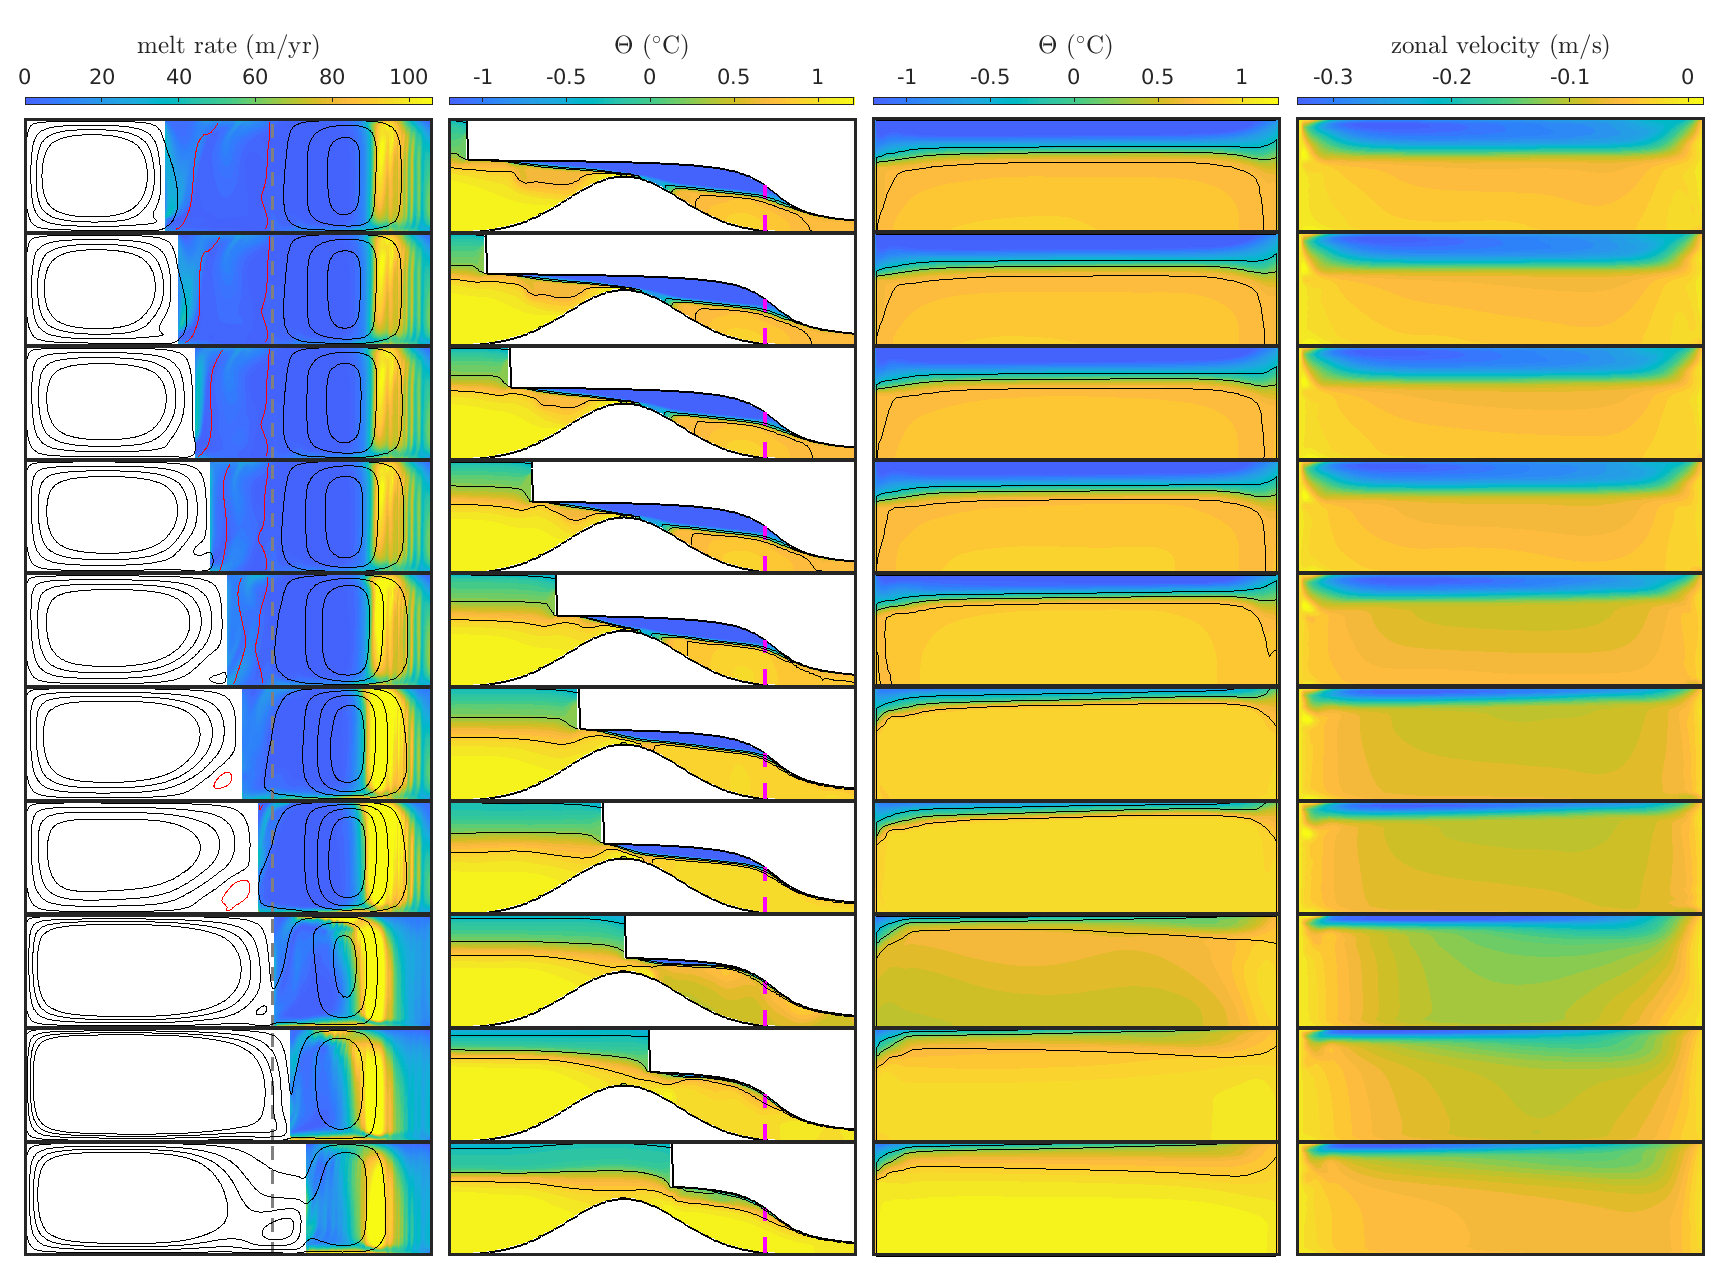
\includegraphics[width = 0.99\textwidth]{../make_figures/plots/figure5.eps}
    \caption{columns showing (a) change of melt rate with snap, (b) meridional cross sectio T and S, (c) zonal cross section T and S, (d) zonal velocity zonal cross section. \red{add a,b,c,d labels for columns and arrow along left with $l_c$}}
    \label{fig:figure5}
\end{figure}

%how can we understand what happens.
To understand why the changes in thermal driving and boundary layer velocity behave as they do, it is instructive to consider the barotropic stream function and zonal and meridional cross sections, shown in figure~\ref{fig:figure5} (for the default run, to which the first row corresponds, these are identical to figure~\ref{fig:figure3}b,e, and d, respectively). These plots indicate that while the ice front is still located beyond the ridge, the strong PV barrier provided by the ridge and ice draft remains and a topographically constrained cyclonic circulation is spun up inshore of the ridge (there is zero barotropic flow across the ridge, see figure~\ref{fig:figure5}, first column), with a strong boundary current at the East of the domain which provides hot water access to the inner cavity, as described in section~\ref{S:Baseline:Default} for the default run. In this case, calving events result in a less prominent meltwater plume (figure~\ref{fig:figure5}, second column), which permits greater warm water access to the inner cavity (figure~\ref{fig:figure5}, third column) because (1) meltwater mixing at the Eastern boundary is reduced and (2) (for larger values of the calved length) the hydrographic front on the north of the ridge reaches the ridge crest and warm water is able to spill over the central portion of the ridge. The increased presence of warm water (both in quantity and temperature) results in increased melting because there is a great quantity of heat available for melting and the topographically constrained circulation is more vigorous, as mentioned above.

When the ice front is calved on top of the ridge, however, their are two important changes. Firstly, the strong PV barrier provided by the ridge crest and ice draft is relaxed, and the domains become connected. The flow within the cavity is still cyclonic (figure~\ref{fig:figure5}, first column), but far less constrained and thus the velocity effect is reduced. The second change, which is related to the first, is that vast amounts of warm water are now able to spill over the ridge, and the inner cavity is entirely flooded with warm water; although this means there is far more heat available for melting (thermal driving effect increases when calving on top of the ridge, figure~\ref{fig:figure4}b), this also results in a reduced stratification and thus reduction in the velocity effect. The two mechanisms that reduce circulation -- reductions in stratification and topographic constraint on the circulation -- outweigh the increase in heat available for melting, resulting in a significant reduction in the heat available for melting.


%We gain insight into why the velocity and thermal driving effects behave as described by considering the barotropic stream function and cross sections shown in figure~\ref{fig:figure5}. 
%\begin{itemize}
%    \item When the front is located beyond the ridge, further calving events do not change the topographic barrier provided by the ridge and so the inner cavity circulation still dominated by a strongly confined cyclonic circulation (first column)
%    \item However, snapping in this case reduces the area of the plume (second column), as it is constrained to satisfy the geometry. 
%    \item This means that mixing along the boundary wall where warm water enters is reduced, meaning less modified (i.e. warmer) water entering cavity (third column). NB. still little flow over the ridge proper. 
%    \item This means that (a) water is warmer in the inner cavity (i.e. more thermal driving) and (b) stronger stratification (third column) which enhances vigour of circulation (i.e. more velocity effect).
%    \item When we snap to the ridge crest, two things happen  (1) The pv barrier provided by the ridge crest/ice shelf is relaxed and the circulation connect with one another. The circulation is no longer so strongly confined and thus reduces speed (see column 4, reduce velocity effect). (2): In addition to connected domains meaning more heat access, plume no longer blocks ridge crest (it no longer extends that far!); both of these mean that inner cavity flooded with essentially unmodified cdw. This means that there is more heat available for melting (thermal driving effect increases), but also reduced stratification (reduce velocity effect).
%\end{itemize}



\section{Effect of Cavity Geometry on Melt Response to Calving}\label{S:Results:H}
%what are we doing here and why (briefly)
In the previous section, we analyzed how, and why, the inner cavity melt rate changes with calving in the $H$=100~m case. The strength of the topographic barrier provided by the seabed ridge in combination with the ice draft was identified as a important control on the melt rate response to calving; in this section, we describe how this picture changes for larger values of $H$ ($H$ = 150~m and $H$=200~m), and the strength of the topographic barrier is therefore reduced.

%how do melt rates change
The inner cavity melt rate and as a function of the calved length $l_c$ and velocity-thermal driving decomposition are plotted in figure~\ref{fig:figure6} for both $H$ = 150~m and $H$ = 200~m. Comparison with the corresponding results for $H$=100~m (figure~\ref{fig:figure6}a) indicates that at larger values of $H$, the change in inner cavity melt rate is far less sensitive to calving: the range of inner cavity melt rates reduces from approximately 25\mpryr for $H$=100~m to 10\mpryr and 7\mpryr for $H$=150~m and $H$=200~m, respectively. In addition, the peak inner cavity melt rate is reached when the ice extent is greater ($l_c$ is smaller) as the gap $H$ is reduced: the value of $l_c$ at which the highest inner cavity melt rate is realised is approximately 29~km, 14~km, and 10~km for $H$=100~m, 150~m, and 200~m, respectively.

Despite these differences, there are parallels to be drawn between these cases...

\begin{figure}
    \centering
    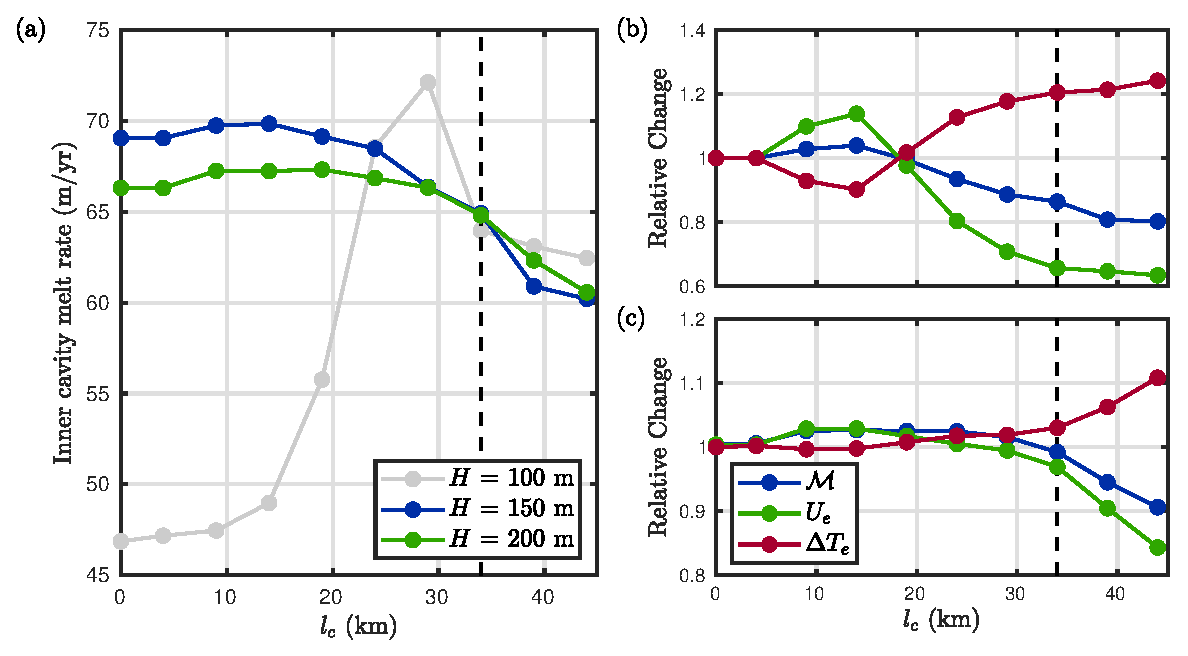
\includegraphics[width = \textwidth]{../make_figures/plots/figure6.eps}
    \caption{(a) Inner cavity melt rate as a function of the calved length $l_c$ for $H$=100~m (light grey, as in figure~\ref{fig:figure4}a), $H$=150~m (blue), and $H$=200~m (green). The black dashed line indicates the position of the ice front when it is located directly above the seabed ridge. (b)-(c) Velocity-thermal driving decomposition for (b) $H$ = 150~m and (c) $H$ = 200~m: plot of the decomposition of changes in inner cavity melt rate relative to the default (uncalved) experiment (equation~\eqref{E:MillgateDecompMelt}) into changes in boundary layer speed $U_\text{effect}$ (green curve, equation~\eqref{E:MillgateDecompU}) and thermal driving $\Delta T_{\text{effect}}$ (red curve, equation~\eqref{E:MillgateDecompDT}).}
    \label{fig:figure6}
\end{figure}

\begin{figure}
    \centering
    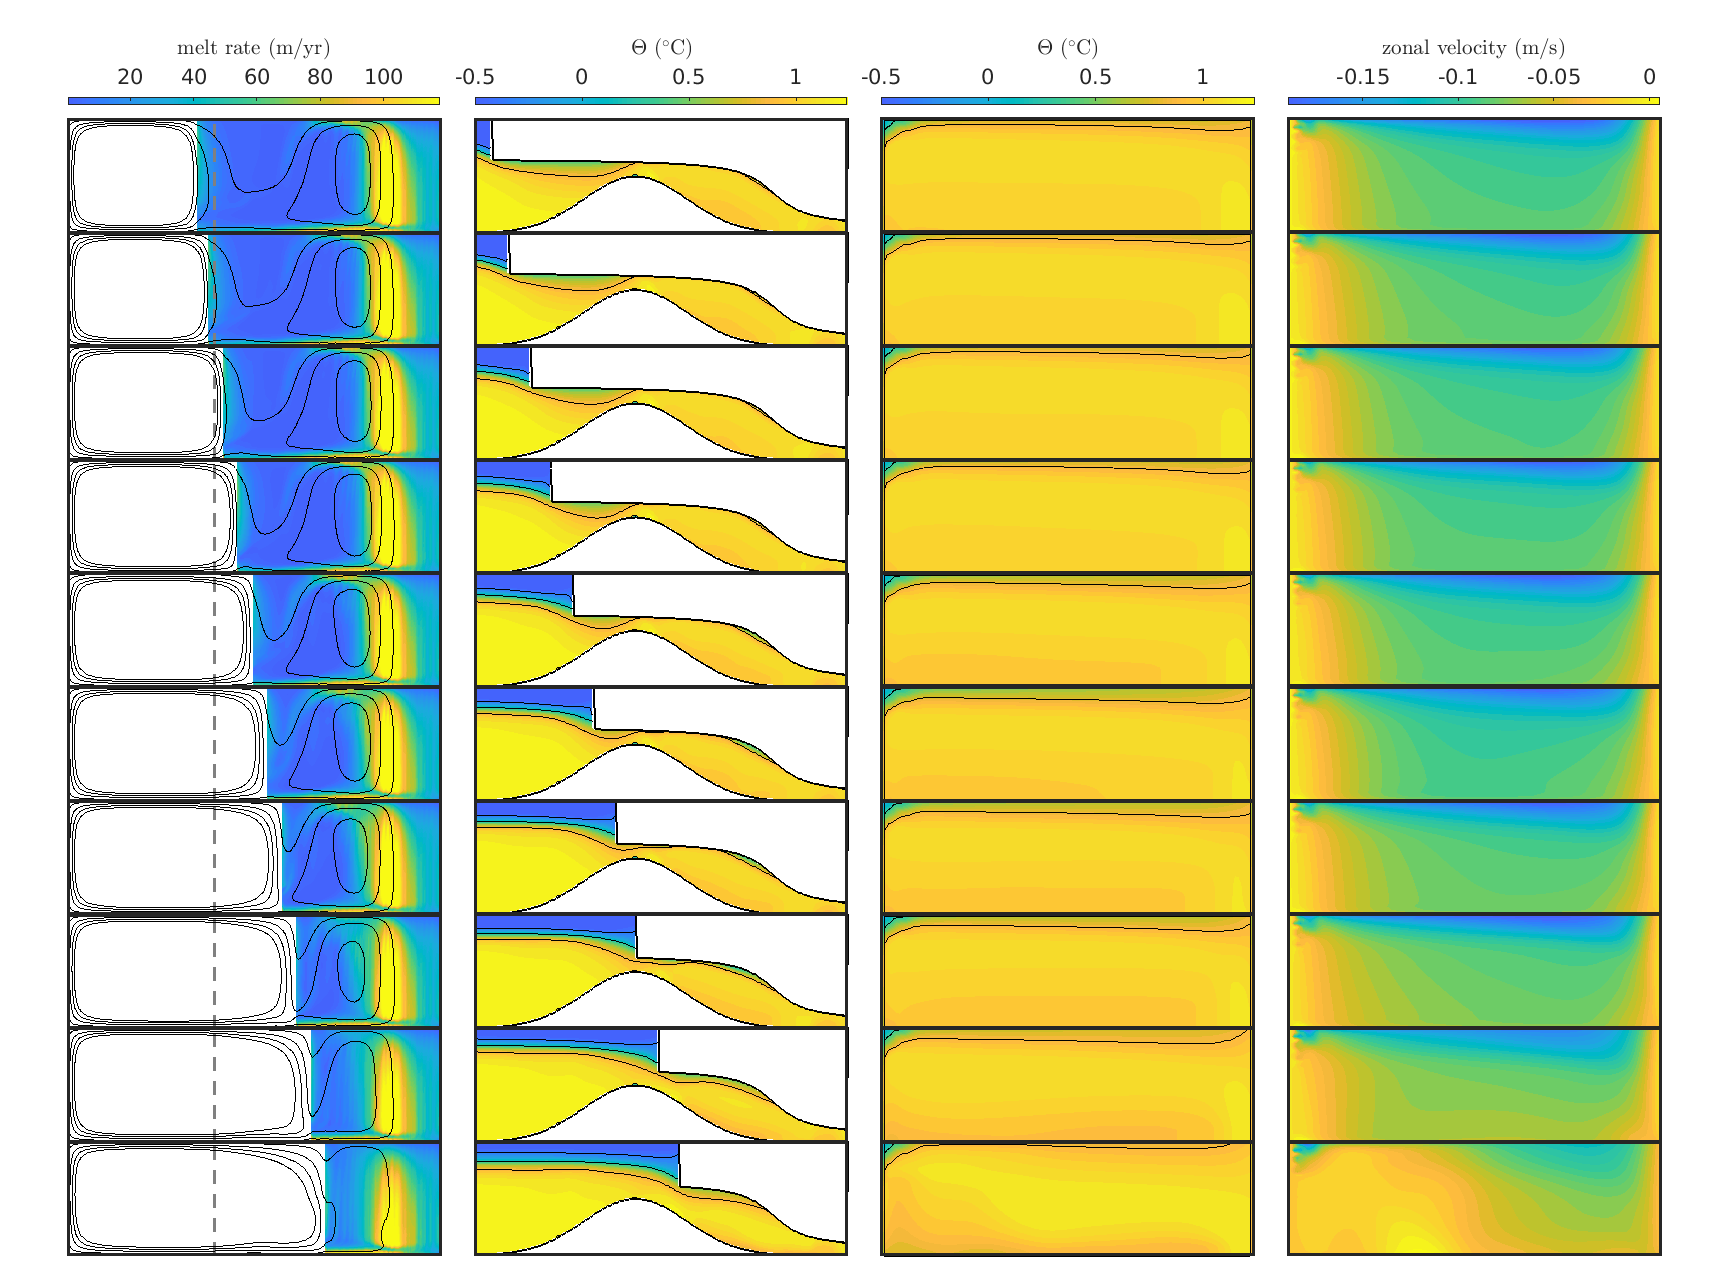
\includegraphics[width = \textwidth]{../make_figures/plots/figure7.eps}
    \caption{Columns as in figure 5 for W = 200 case (note different colour bars in second and third column). \red{needs a,b,c,d labels}}
    \label{fig:figure7}
\end{figure}


%what do we see
Mean melt rates as a function of calved length for the two larger gaps we consider here ($W = 150$~m and $W = 200$~m) are plotted in figure~\ref{fig:figure6}. As in the $W = 100$ case, we see that the melt rate reaches a peak while the ice front is located north of the ridge crest, and further calving events beyond this point reduce the melt rate. From the decomposition, we see in both cases that a reduction in the cavity circulation that outweighs an increase in thermal driving is responsible (and both relative changes are a similar order of magnitude) for the reduction in mean inner cavity melt rate beyond this point.  However, there are several important differences: firstly, the inner cavity melt rate is far less sensitive to calving in both the $W = 150$ and $W = 200$m cases (the difference between largest and smallest inner cavity melt rates is approximately 20\% and 10\%, respectively), and follows the upper end of the maximum range seen in the $W = 100$m case; secondly, the inner cavity melt rate does not show any sort of threshold behaviour when the calving front reaches the top of the ridge.

%why do we see it
To understand the reasons it is useful to compare the cross sections in figure~\ref{fig:figure4} for the $W = 100$ case to the corresponding plot in figure~\ref{fig:figure7} for the $W = 200$ case (a comparison between the $W = 100$m and $W = 150$m case is qualitatively similar to that discussed below for $W = 100$, but the differences are clearer for $W = 200$m.)
%\begin{itemize}
%    \item Domains are connected even in the default run, and the inner cavity is entirely flushed with warm water. This is different to the `fully' calved $W = 100$m case because the ridge still provides a strong pv barrier constraining the flow to the inner cavity and strongly bounding it, permitting high velocities necessary to allow high mean melt rates.
%
%\end{itemize}


\section{Effect of Hydrographic Conditions on Melt Response to Calving}\label{S:Results:P}
Before moving on to assess how melt rates change with calving in realistic simulations of Pine Island, we briefly consider how the picture presented in the previous two sections depends on the choice of hydrographic conditions to which the ocean state is restored far from the ice shelf.

% Introduce simulations with reminder of what they correspond to 
In figure~\ref{fig:figure8}, we present the inner cavity melt rate and velocity-thermal driving decomposition for experiments 4--9 (table \red{tabref}), which cover the three geometric values ($W$ = 100~m, $W$ = 150~m, and $W$ = 200~m) for $P$=700 (dashed profile in figure~\ref{fig:figure2}, experiments 4--6) and $P$=800 (dot-dashed profile in figure~\ref{fig:figure2}, experiments 7--9). Recall that the $P$=800 cases approximately corresponds to observations in Pine Island Bay in 2012, when the thermocline was at one of the lowest values on record. As mentioned, we consider a constant ridge height and thus variability in the difference between the lower layer depth and height of the ridge -- which is thought to be the key driver of the amount of CDW able to spill over the ridge -- is entirely captured by the variability in the value of $P$.

\begin{figure}
    \centering
    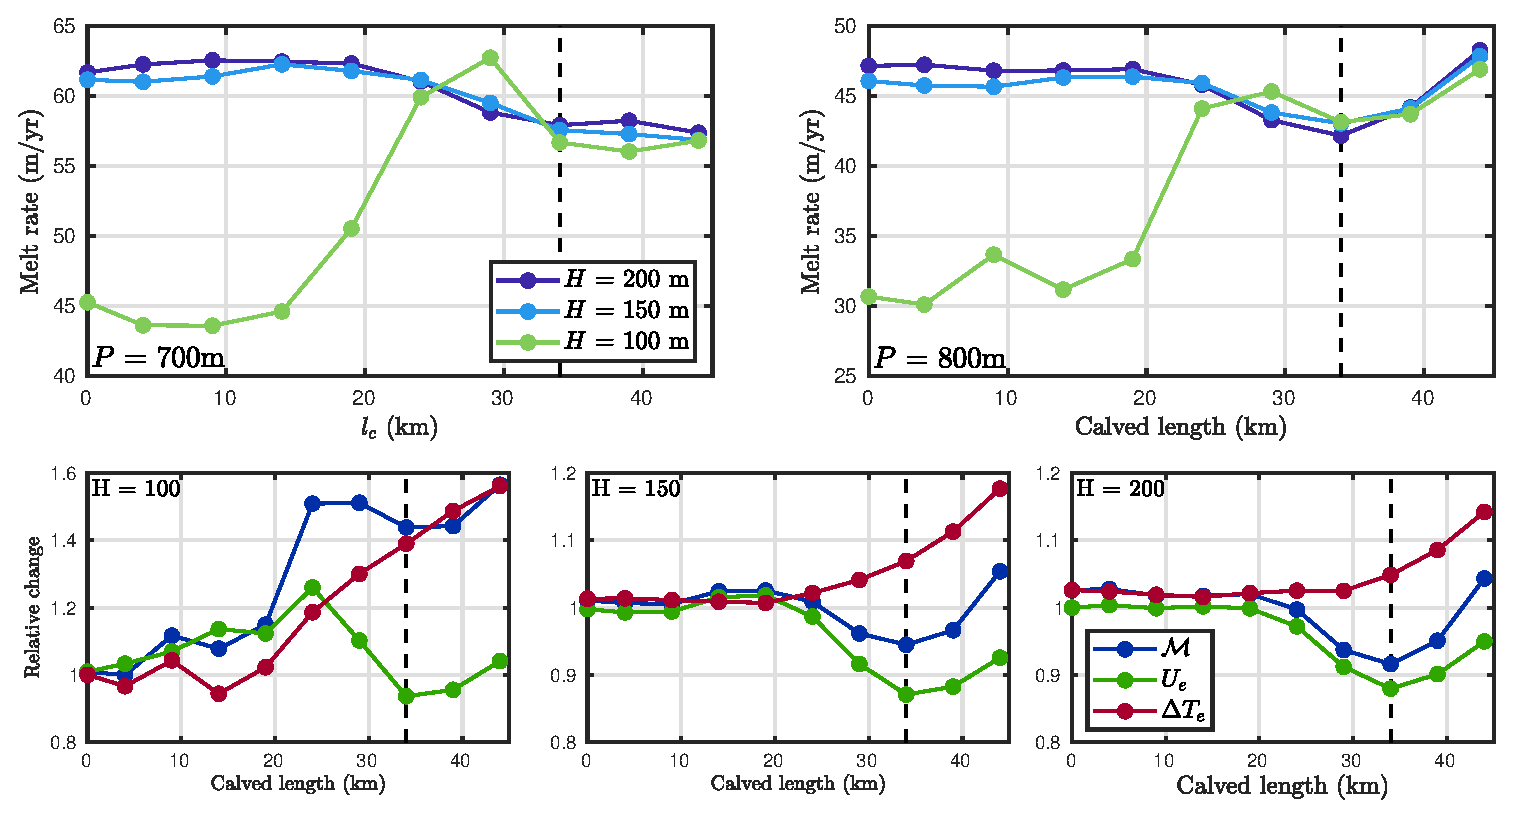
\includegraphics[width = \textwidth]{../make_figures/plots/figure8.eps}
    \caption{(a)--(b) Inner cavity melt rate as a function of calved length $l_c$ in idealized Pine Island simulations with (a) $P$=700~m and (b) $P$=800~m. Colours correspond to different values of $W$, as indicated by the legend in (a). The black dashed line indicates the location of the crest of the sea-bed ridge. (c)--(e) Velocity--thermal driving decompositions (as in figure~\ref{fig:figure4}) for the the data shown in (b): (c), (d), and (e) correspond to the results for $W$=100~m, $W$=150~, and $W$=200~m, respectively, as indicated. }
    \label{fig:figure8}
\end{figure}

% Brief results for P = 700 (very similar to the P = 800 case)
The results for $P$=700~m are very similar to those for $P$=800~m, albeit with slightly lower melt rates. The result can be summarized as for the $P$=800~m case: for the narrowest gap ($W$=100~m), the inner cavity melt rate is very sensitive to the front position; it increases rapidly with calving as the calving front approaches the ridge, before dropping off sharply when the ice front reaches the top of the ridge and stabilizing for further calving events. For the wider gaps ($W$=150~m, $W$=200~m), the melt rates are far less sensitive to changes in ice front position, reaching a peak when the ice front is some way upstream of the ridge (figure~\ref{fig:figure8}) and decrease steadily with further calving events. The velocity-thermal driving decompositions for the experiments with $P$=700~m (not shown) reveal that, as in the $P$=800~m case, these observations can be explained by the competition between velocity changes owing to stratification and communication between the inner and outer cavities, and the increased heat available for melting in the inner cavity. As mentioned, the relationship between the CDW layer depth and the height of the ridge is expected to be the important control; when framed in this way, the similarity between the $P$=800~m and $P$=700~m cases is unsurprising: in both of these, the CDW layer extends all the way to the top of the ridge (figure~\ref{fig:figure2}).

%results are different for P = 800 -- how?
In the $P$=800~m case, however, the CDW layer does not extend all the way to the top of the ridge (figure~\ref{fig:figure2}). In this case, the melt rate increases with calving at while the ice front is located downstream of the ridge, as in the $P$=700~m cases and the melt rate drops off when the ice front reaches the top of the ridge that is associated with a reduction in boundary layer velocity (figure~\ref{fig:figure8}) -- the inner and outer cavities are able to talk to one another. However, unlike the $P$=700~m cases, subsequent calving events result in an increase in inner cavity melt rate that is associated with an increase in boundary layer velocity. The crucial difference here is that once the calving front has reached the top of the ridge, the fact that the CDW layer is below the top of the ridge means that a strong topographic barrier still exists and, unlike in the other two cases, the inner cavity is not entirely flushed with CDW. Further calving events thus increase the stratification further (rather than reducing it, as is the case for an entirely flushed cavity), leading to a strengthening of the circulation. 


\begin{figure}
    \centering
    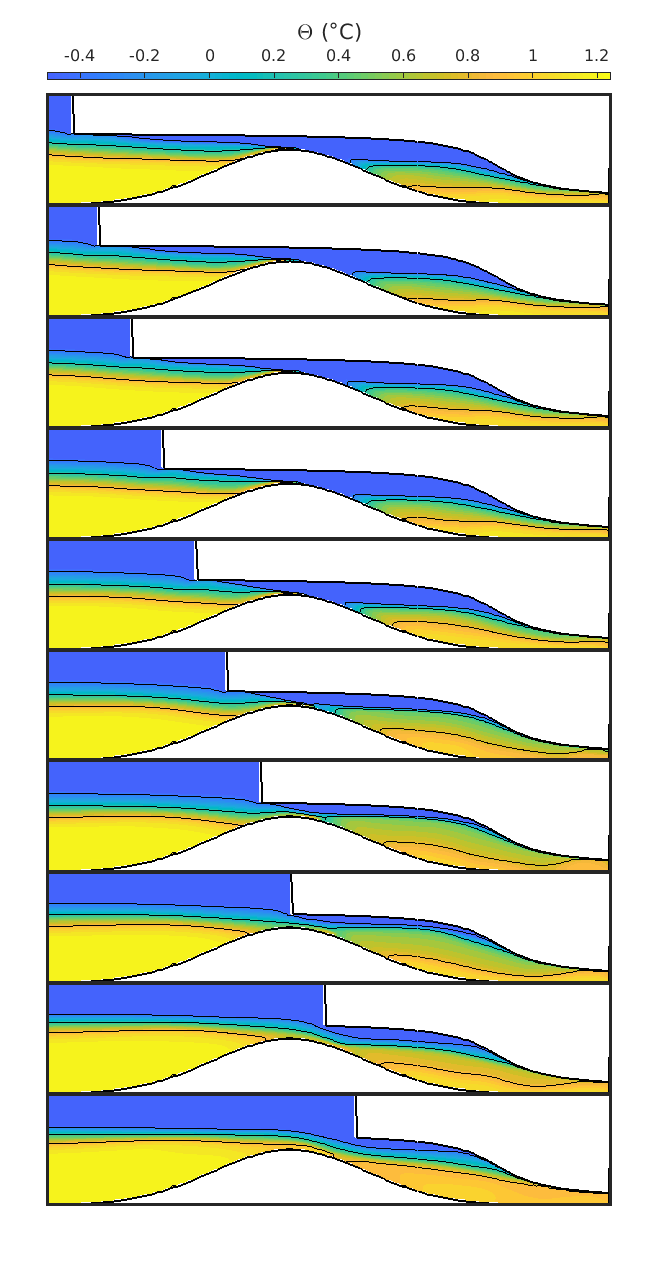
\includegraphics[width = 0.35\textwidth]{../make_figures/plots/figure9.eps}
    \caption{figure 9: meridional ridge cross sections for the $P$=800~m case (will be to the side c.f. figure 7 in JDR 2014 paper) }
    \label{fig:figure9}
\end{figure}


\section{Pine Island Simulations}
% intro to the section
The idealized modelling reveals how melt rates near the grounding line are expected to respond to calving events in a cavity with a seabed ridge that is uniform in the zonal direction. We now turn to results for the realistic Pine Island Cavity, and use these idealized results to guide our understanding of the results in this case. 

\begin{figure}
    \centering
    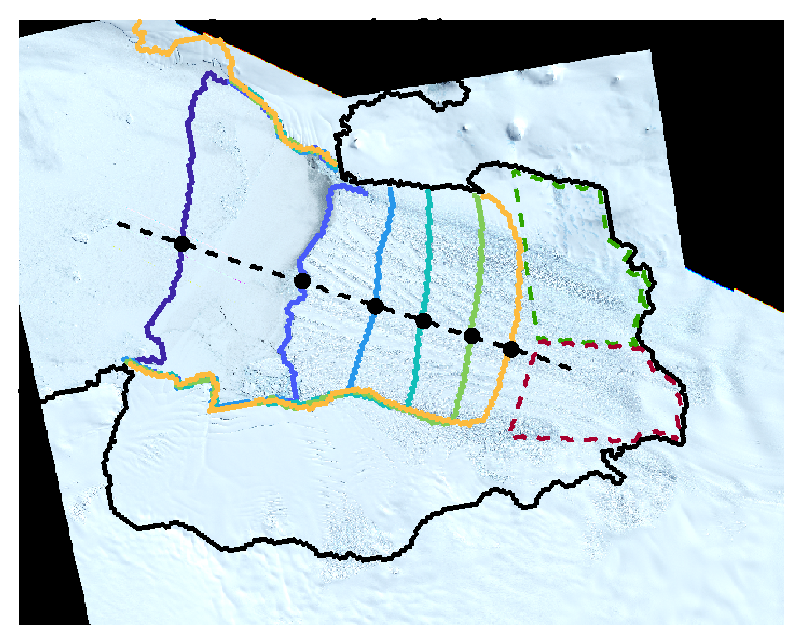
\includegraphics[width = 0.75\textwidth]{../make_figures/plots/figure10.eps}
    \caption{Ice front positions in realistic Pine Island simulations. Purple to yellow colormap curves indicate the six ice front positions used in realistic Pine Island experiments, with dark purple corresponding to the 2009 front and blue corresponding to the 2020 front position (see main text). The solid black line indicates the 2009 grounding line position from~\cite{Joughin2010GRL}. The black dashed line roughly indicates the centreline of the cavity, along which the calved length is measured, while the blue dashed line approximately indicates  the peak of the sea bed ridge (corresponding to the black dashed line in figure~\ref{fig:figure1}. The green (North) and red (South) boxes indicate the inner cavity regions considered in the experiments. Inset: plot of the vertical gap between the ridge crest and the ice draft, measured northwards along the blue dashed line in the main figure. Red and green shaded sections roughly correspond to locations immediately upstream of the red and blue boxes in the main figure, respectively. The background image is a Sentinel 2 mosaic from November 2020. \red{add lat/lon lines as grid? Add A, B labels as in figure 1. Add Northern box/Southern box labels}}
    \label{fig:figure10}
\end{figure}

%Describe experiments
\subsection{Experiment Details}
To assess the effect of calving events on the sub-shelf melting in Pine Island Glacier, we resolve the cavity circulation using the same ocean model as described in \S\ref{S:Experiment:Model} with six different ice shelf topographies, as shown schematically in figure~\ref{fig:figure10}: the first two simulations (purple and blue ice fronts in figure~\ref{fig:figure10}) represent realistic situations with ice shelf positions corresponding to 2009 and 2020 conditions, and the four further simulations use the same topography with sections of fast flowing ice removed. Note that the ice thickness, and thus grounding line position and ice shelf draft, at remaining shelf locations remains the same in each simulation. Consistently with the idealized simulations, we refer to the simulation with the 2009 ice front as the default run.

%how do we get cavity and draft
The sub shelf cavity is computed from the ice and seabed geometry, which we take from~\citeA{Dutrieux2014Science}. Briefly, the ice shelf geometry is calculated from a 40~m-resolution digital elevation model of the ice freeboard from 2008~\cite{Korona2009Photogrammetry}, that is adjusted with a constant medium bias from observations obtained from the Autosub underwater autonomous vehicle~\cite{Jenkins2010NatureGeo}. The DEM assumes freely floating ice throughout the shelf, which may reduce its accuracy close to the grounding line. Over the continental shelf, the seabed geometry is well known from ship echo-sounding \cite{Dutrieux2014Science}, while in the cavity it calculated from an inversion of gravimetry data and corrected point-wise using the median difference between the depth from the gravimetry inversion and from the Autosub observations. 

%model notes and calibration
We consider a single hydrographic forcing, corresponding to observed 2009 conditions in Pine Island Bay (dark grey line in figure~\ref{fig:figure2}b,c). All model parameters are as described in \S\ref{S:Experiment:Model}, with the exception of the drag coefficient that enters into the three-equation formulation implementation of melting; this parameter is tuned to 4.5$\times10^{-3}$ to approximately match the estimated total meltwater flux in 2009 (80 km\textsuperscript{3}/yr)~\cite{Dutrieux2014Science}). The simulated melt rate for the baseline simulation with the 2009 ice shelf geometry (figure~\ref{fig:figure11}a) is consistent with observations (not shown), displaying complex features on small scales, but characterized on larger scales as being concentrated near to the grounding line, with a peak melt rate of 120~m~yr\textsuperscript{-1}.

%gap is not uniform, but sort of split. Tell the reader what the different regions are.
As mentioned in \S\ref{S:Introduction}, in the realistic case, the ridge-draft gap is not uniform but varies from 100~m at its narrowest to 400~m at its widest; this range motivated the choice of gap thicknesses $W$ in the idealized simulations. The ridge-draft gap (inset in figure~\ref{fig:figure10} can be approximately partitioned into two sections: in the Southern part of the cavity (red shading on inset of figure~\ref{fig:figure10}), the gap is relatively wide (average width \red{x}), while in the Northern part of the cavity (green shading) the gap is narrow (average width \red{x}); to facilitate inferences from our idealized results -- with a uniform ridge-draft gap -- to be made, we evaluate changes in melting with calving in two regions upstream of these two halves, indicated by the red and green boxes in figure~\ref{fig:figure10}. \red{caveat here that the two regions are connected!}

\subsection{Results}

\begin{figure}
    \centering
    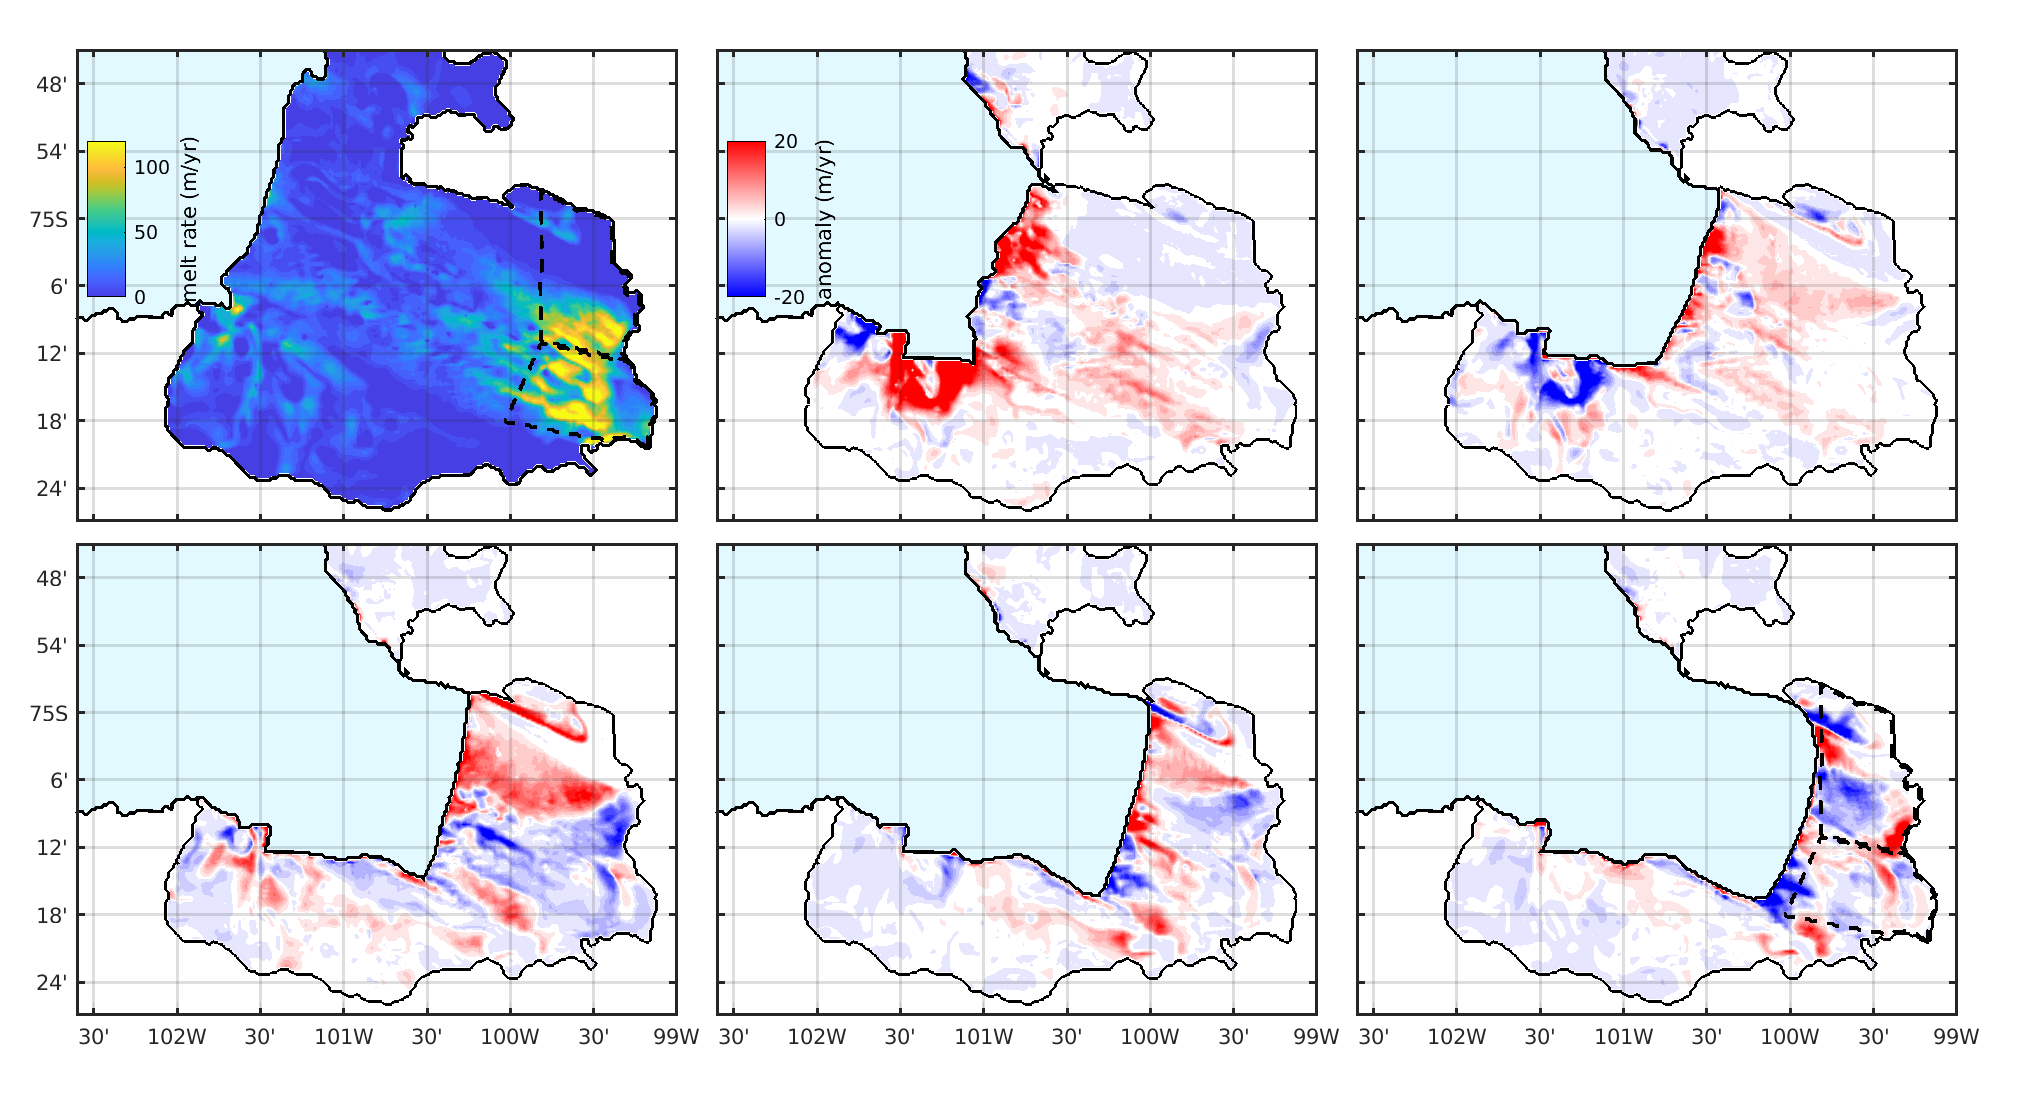
\includegraphics[width = \textwidth]{../make_figures/plots/figure11.eps}
    \caption{(a) Simulated melt rate in Pine Island with 2009 ice front. Black dashed boxes indicate the North and South boxes (see figure~\ref{fig:figure10}), where the highest melt rates are concentrated. (b)--(f) Non-cumulative melt rate anomaly in the simulations (i.e. measured relative to the previous panel). The colourbar in (b) is appropriate for each of (b)--(f). In each case, ice shelf front and grounding line (2009 grounding line position from ~\cite{Joughin2010GRL}) are shown as a solid black line. \red{Add the ridge dashed line and a scale bar here.}} 
    \label{fig:figure11}
\end{figure}


%introduce simulations
Figure~\ref{fig:figure11} contains a plot of the melt rate over the whole cavity for the default run, and the non-cumulative melt rate anomalies for the other five ice front positions. To be explicit, red (blue, respectively) locations on these maps indicate areas in which the melt rate has increased (decreased) when the ice front was latest section of the ice shelf was removed, rather than being measured relative to the default run. 

%Melt rates look qualitatively similar in the default run to the idealized case
The pattern of melt rates in the default case is qualitatively similar to the corresponding idealized simulation in the idealized case: melt rates peak are concentrated near to the grounding line, reaching a peak of approximately 120~\mpryr several kilometers downstream of it, while the melt rate in the majority of the shelf is below 20~\mpryr. In addition, melt rates are slightly higher on the Coriolis favoured Western boundaries, although this picture is complicated by the oblique orientation of Pine Island, and the complex geometry of both the ice shelf base and seabed.

%2009--now: large anomalies at the front
When the ice front is retreated from its 2009 position to its present day (2020) position, melt rates within 10~km of the ice front increase significantly along its whole length. This affect is attributed to high velocities associated with upwelling at the new ice shelf front as well as the formation of a gyre in the embayment in the newly open ocean where ice was present in the baseline geometry, but not in 2020 (not shown) \red{cite Seung-Tae's paper!]}: this gyre results in a strong circulation along the ice shelf front (the ice shelf front is a dynamic barrier to flow and provides a freshwater source to enhance the flow). These large anomalies at the ice shelf front are expected to lead to significant local thinning, which may encourage further calving events (the critical cliff height for collapse is thought to be strongly dependent function on the height of the cliff~\cite{Crawford2021NatureComms}). 

%2009-now: small changes in the inner cavity region
Melt rates do not change significantly, however, in the inner cavity regions, when the ice front is retreated from its 2009 position to its current (2020) position: the average melt rate in the Northern and Southern boxes increase by approximately 1\mpryr and 2\mpryr respectively (figure~\ref{fig:figure12}a). \red{Need to say something about the implications of this.}

%Qualitative descriptions of melt anomalies: (a) characterized by complex patterns, (b) only see significant changes when calving beyond the ridge (large positive anomaly in the northern shear margin which might be important for stability), (d) melt rates decrease when ice front has retreated significantly (this is a lead in to the qualitative analysis of fig 12)
Melt rate anomalies in the `future' experiments display complex patterns, featuring large regions of both positive and negative anomalies in each case (figure~\ref{fig:figure11}). Despite these complex patterns, there are several features to note: firstly, with the exception of a large negative anomaly in the Southern shear margin, melt rates anomalies do not display signifcant changes in the first 'future' snap, suggesting a reasonable `safety band' for changes in melt rate with calving. \red{don't like this phrasing: I mean that, we won't see large changes until a more significant area has calved}. Secondly, however, melt rates around the Northern shear margin increase significantly when the ice front is retreated to lie (approximately) above the seabed ridge (figure~\ref{fig:figure11}d). This region of enhanced melt rates extends almost all the way to the grounding line. The shear margins of PIIS play an important role in buttressing the grounded ice~\cite{Lhermitte2020PNAS}; enhanced thinning of these regions may reduce buttressing and thus increase ice losses from the grounded ice. \red{Do you want to say something about that we're closer to this situation that the 2009 situation..?}. Finally, melt rates decrease significantly over large areas of the ice shelf when the front is retreated a significant distance upstream of the ridge (figure~\ref{fig:figure11}f).

\begin{figure}
    \centering
    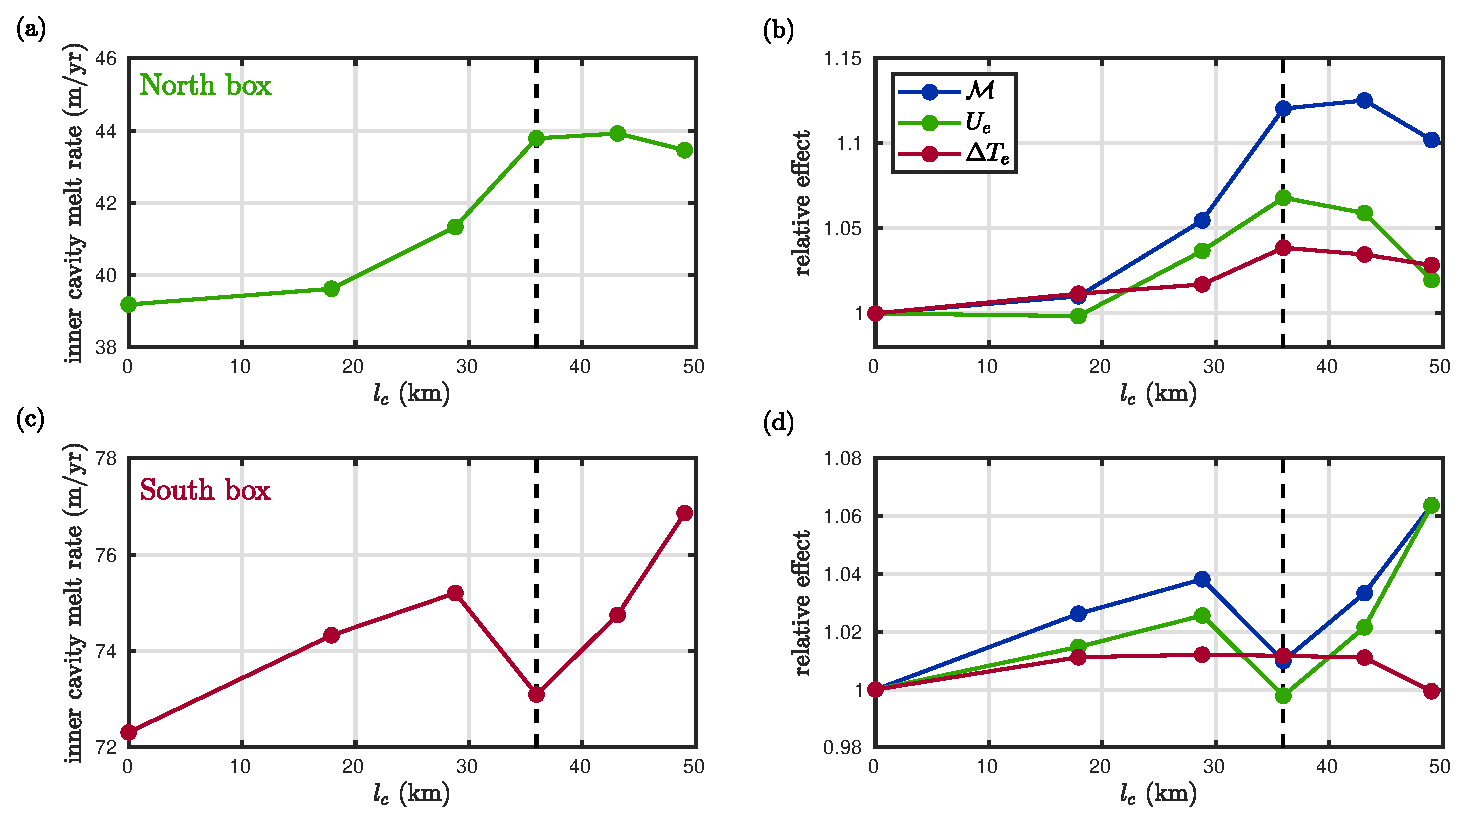
\includegraphics[width = \textwidth]{../make_figures/plots/figure12.eps}
    \caption{(a), (c) Average melt rate as a function of calved length $l_c$ in realistic simulations of Pine Island. Plots (a) and (c) correspond to the North (green dashed) and South (red dashed) boxes shown in figure~\ref{fig:figure10}, respectively. The calved length $l_c$ is the distance measured along the black dashed line in figure~\ref{fig:figure10}, taken relative to the 2009 ice front position (purple curve in figure~\ref{fig:figure10}.). (b), (d) Velocity-thermal driving decomposition for the changes in melt rate shown in (a) and (c), respectively. As indicated by the legend in (b) and (d), blue, red, and green curves correspond to simulated changes $\mathcal{M}$, velocity effects $U_e$, and thermal driving effects $\Delta T_e$, respectively. In all plots, the black dashed line approximately corresponds to the location of the peak of the ridge along the black dashed line in figure~\ref{fig:figure10}, where it intersects with the blue dashed line. \red{Perhaps label 2009 and 2020 in (a) and (c)}}\label{fig:figure12}
\end{figure}

%these qualitative observations sort of agree with the mean melt rate plots
These qualitative observations are borne out in plots of the mean melt rate as a function of calved length, shown in figure~\ref{fig:figure12}. In the Northern box, mean melt rates remain approximately constant until the ice front approaches the seabed ridge and they increase quickly. When the ice front is retreated further, melt rates reduce weakly. In the Southern box, melt rates increase while the ice front is located downstream of the seabed ridge, before dropping temporarily when the ice front is retreated to the ridge and subsequently increasing again. 

%northern box 'hides' behind a narrow gap -- make comparison with the narrow idealized case
Our interpretation of these results is facilitated by the idealized simulations presented in \S\ref{S:Baseline}--\ref{S:Results:P}. The Northern box `hides behind' a relatively narrow gap between the seabed ridge and the ice draft (see inset in figure~\ref{fig:figure10}), and the change in melt rates with calving behaves in a qualitatively similar manner to idealized results with narrow ($W$=100~m, $W$=150~m) gaps. In addition, a velocity-thermal decomposition of these changes in melt rates indicates that -- as in the corresponding idealized case -- both enhancement in thermal driving and velocity contributions of a similar magnitude are responsible for the changes while the ice front is located downstream of the ridge, while a reduction in the velocity effect is responsible for the weak decrease when calving beyond the ridge. In the idealized case, the reduction in velocity effect when calving beyond the ridge was much stronger, and the decrease in melt rate therefore much larger, than in this realistic case; we attribute this difference to the splitting of a connected domain into two sub-regions, and the particular complexities of the realistic cavity.

%southern box 'hides' behind a wide gap -- make comparison with the wide idealized case
In contrast, the Southern box `hides behind' a relatively wide gap between the seabed ridge and the ice draft. As was the case for idealized simulations with wide ($W \gtreq$200~m), the mean melt rate is approximately independent of calving (the difference between the minimum and maximum melt rates in the Southern box is approximately 6\%, which is almost half of the corresponding value in the Northern box). It is interesting to note that the slight trend on top of this constant value -- with a drop of in melt rates when the ice front is located on top of the ridge, associated with a reduction in velocities, that is reversed under further calving (figure~\ref{fig:figure12} --  is similar to idealized results with a lower pycnocline (see figure~\ref{fig:figure8}(b)--(e)). Drawing analogy to the idealized cases, this suggests that the hydrography in the Southern cavity is not entirely saturated, and significant calving continues to increase stratification in this region, unlike in the Northern box, which is entirely flushed with warm water. \red{this is \textit{tenuous}! But it would be good to shoehorn in a comparison with idealized that goes beyond invariance}



\section{Discussion}\label{S:Discussion}
Discussion points:
\begin{itemize}
    \item Changes in melt rate not as large as in the idealized case -- but still significant, particularly those at the ice front and possibly at the shear margins.
    \item There is uncertainty in the ridge gap (and in the future ice might advect downstream to close the gap), meaning that future responses to calving are larger than we predict here.
\end{itemize}
\section{Summary and Conclusions}



%%% Suggested section heads:
% \section{Introduction}
%
% The main text should start with an introduction. Except for short
% manuscripts (such as comments and replies), the text should be divided
% into sections, each with its own heading.

% Headings should be sentence fragments and do not begin with a
% lowercase letter or number. Examples of good headings are:

% \section{Materials and Methods}
% Here is text on Materials and Methods.
%
% \subsection{A descriptive heading about methods}
% More about Methods.
%
% \section{Data} (Or section title might be a descriptive heading about data)
%
% \section{Results} (Or section title might be a descriptive heading about the
% results)
%
% \section{Conclusions}


%Text here ===>>>


%%

%  Numbered lines in equations:
%  To add line numbers to lines in equations,
%  \begin{linenomath*}
%  \begin{equation}
%  \end{equation}
%  \end{linenomath*}



%% Enter Figures and Tables near as possible to where they are first mentioned:
%
% DO NOT USE \psfrag or \subfigure commands.
%
% Figure captions go below the figure.
% Table titles go above tables;  other caption information
%  should be placed in last line of the table, using
% \multicolumn2l{$^a$ This is a table note.}
%
%----------------
% EXAMPLE FIGURES
%
% \begin{figure}
% \includegraphics{example.png}
% \caption{caption}
% \end{figure}
%
% Giving latex a width will help it to scale the figure properly. A simple trick is to use \textwidth. Try this if large figures run off the side of the page.
% \begin{figure}
% \noindent\includegraphics[width=\textwidth]{anothersample.png}
%\caption{caption}
%\label{pngfiguresample}
%\end{figure}
%
%
% If you get an error about an unknown bounding box, try specifying the width and height of the figure with the natwidth and natheight options. This is common when trying to add a PDF figure without pdflatex.
% \begin{figure}
% \noindent\includegraphics[natwidth=800px,natheight=600px]{samplefigure.pdf}
%\caption{caption}
%\label{pdffiguresample}
%\end{figure}
%
%
% PDFLatex does not seem to be able to process EPS figures. You may want to try the epstopdf package.
%

%
% ---------------
% EXAMPLE TABLE
%
% \begin{table}
% \caption{Time of the Transition Between Phase 1 and Phase 2$^{a}$}
% \centering
% \begin{tabular}{l c}
% \hline
%  Run  & Time (min)  \\
% \hline
%   $l1$  & 260   \\
%   $l2$  & 300   \\
%   $l3$  & 340   \\
%   $h1$  & 270   \\
%   $h2$  & 250   \\
%   $h3$  & 380   \\
%   $r1$  & 370   \\
%   $r2$  & 390   \\
% \hline
% \multicolumn{2}{l}{$^{a}$Footnote text here.}
% \end{tabular}
% \end{table}

%% SIDEWAYS FIGURE and TABLE
% AGU prefers the use of {sidewaystable} over {landscapetable} as it causes fewer problems.
%
% \begin{sidewaysfigure}
% \includegraphics[width=20pc]{figsamp}
% \caption{caption here}
% \label{newfig}
% \end{sidewaysfigure}
%
%  \begin{sidewaystable}
%  \caption{Caption here}
% \label{tab:signif_gap_clos}
%  \begin{tabular}{ccc}
% one&two&three\\
% four&five&six
%  \end{tabular}
%  \end{sidewaystable}

%% If using numbered lines, please surround equations with \begin{linenomath*}...\end{linenomath*}
%\begin{linenomath*}
%\begin{equation}
%y|{f} \sim g(m, \sigma),
%\end{equation}
%\end{linenomath*}

%%% End of body of article

%%%%%%%%%%%%%%%%%%%%%%%%%%%%%%%%
%% Optional Appendix goes here
%
% The \appendix command resets counters and redefines section heads
%
% After typing \appendix
%
%\section{Here Is Appendix Title}
% will show
% A: Here Is Appendix Title
%
%\appendix
%\section{Here is a sample appendix}

%%%%%%%%%%%%%%%%%%%%%%%%%%%%%%%%%%%%%%%%%%%%%%%%%%%%%%%%%%%%%%%%
%
% Optional Glossary, Notation or Acronym section goes here:
%
%%%%%%%%%%%%%%
% Glossary is only allowed in Reviews of Geophysics
%  \begin{glossary}
%  \term{Term}
%   Term Definition here
%  \term{Term}
%   Term Definition here
%  \term{Term}
%   Term Definition here
%  \end{glossary}

%
%%%%%%%%%%%%%%
% Acronyms
%   \begin{acronyms}
%   \acro{Acronym}
%   Definition here
%   \acro{EMOS}
%   Ensemble model output statistics
%   \acro{ECMWF}
%   Centre for Medium-Range Weather Forecasts
%   \end{acronyms}

%
%%%%%%%%%%%%%%
% Notation
%   \begin{notation}
%   \notation{$a+b$} Notation Definition here
%   \notation{$e=mc^2$}
%   Equation in German-born physicist Albert Einstein's theory of special
%  relativity that showed that the increased relativistic mass ($m$) of a
%  body comes from the energy of motion of the body—that is, its kinetic
%  energy ($E$)—divided by the speed of light squared ($c^2$).
%   \end{notation}




%%%%%%%%%%%%%%%%%%%%%%%%%%%%%%%%%%%%%%%%%%%%%%%%%%%%%%%%%%%%%%%%
%
%  ACKNOWLEDGMENTS
%
% The acknowledgments must list:
%
% >>>>	A statement that indicates to the reader where the data
% 	supporting the conclusions can be obtained (for example, in the
% 	references, tables, supporting information, and other databases).
%
% 	All funding sources related to this work from all authors
%
% 	Any real or perceived financial conflicts of interests for any
%	author
%
% 	Other affiliations for any author that may be perceived as
% 	having a conflict of interest with respect to the results of this
% 	paper.
%
%
% It is also the appropriate place to thank colleagues and other contributors.
% AGU does not normally allow dedications.


\acknowledgments
Enter acknowledgments, including your data availability statement, here.


%% ------------------------------------------------------------------------ %%
%% References and Citations

%%%%%%%%%%%%%%%%%%%%%%%%%%%%%%%%%%%%%%%%%%%%%%%
%
% \bibliography{<name of your .bib file>} don't specify the file extension
%
% don't specify bibliographystyle
%%%%%%%%%%%%%%%%%%%%%%%%%%%%%%%%%%%%%%%%%%%%%%%

\bibliography{mybib}



%Reference citation instructions and examples:
%
% Please use ONLY \cite and \citeA for reference citations.
% \cite for parenthetical references
% ...as shown in recent studies (Simpson et al., 2019)
% \citeA for in-text citations
% ...Simpson et al. (2019) have shown...
%
%
%...as shown by \citeA{jskilby}.
%...as shown by \citeA{lewin76}, \citeA{carson86}, \citeA{bartoldy02}, and \citeA{rinaldi03}.
%...has been shown \cite{jskilbye}.
%...has been shown \cite{lewin76,carson86,bartoldy02,rinaldi03}.
%... \cite <i.e.>[]{lewin76,carson86,bartoldy02,rinaldi03}.
%...has been shown by \cite <e.g.,>[and others]{lewin76}.
%
% apacite uses < > for prenotes and [ ] for postnotes
% DO NOT use other cite commands (e.g., \citet, \citep, \citeyear, \nocite, \citealp, etc.).
%



\end{document}



More Information and Advice:

%% ------------------------------------------------------------------------ %%
%
%  SECTION HEADS
%
%% ------------------------------------------------------------------------ %%

% Capitalize the first letter of each word (except for
% prepositions, conjunctions, and articles that are
% three or fewer letters).

% AGU follows standard outline style; therefore, there cannot be a section 1 without
% a section 2, or a section 2.3.1 without a section 2.3.2.
% Please make sure your section numbers are balanced.
% ---------------
% Level 1 head
%
% Use the \section{} command to identify level 1 heads;
% type the appropriate head wording between the curly
% brackets, as shown below.
%
%An example:
%\section{Level 1 Head: Introduction}
%
% ---------------
% Level 2 head
%
% Use the \subsection{} command to identify level 2 heads.
%An example:
%\subsection{Level 2 Head}
%
% ---------------
% Level 3 head
%
% Use the \subsubsection{} command to identify level 3 heads
%An example:
%\subsubsection{Level 3 Head}
%
%---------------
% Level 4 head
%
% Use the \subsubsubsection{} command to identify level 3 heads
% An example:
%\subsubsubsection{Level 4 Head} An example.
%
%% ------------------------------------------------------------------------ %%
%
%  IN-TEXT LISTS
%
%% ------------------------------------------------------------------------ %%
%
% Do not use bulleted lists; enumerated lists are okay.
% \begin{enumerate}
% \item
% \item
% \item
% \end{enumerate}
%
%% ------------------------------------------------------------------------ %%
%
%  EQUATIONS
%
%% ------------------------------------------------------------------------ %%

% Single-line equations are centered.
% Equation arrays will appear left-aligned.

Math coded inside display math mode \[ ...\]
 will not be numbered, e.g.,:
 \[ x^2=y^2 + z^2\]

 Math coded inside \begin{equation} and \end{equation} will
 be automatically numbered, e.g.,:
 \begin{equation}
 x^2=y^2 + z^2
 \end{equation}


% To create multiline equations, use the
% \begin{eqnarray} and \end{eqnarray} environment
% as demonstrated below.
\begin{eqnarray}
  x_{1} & = & (x - x_{0}) \cos \Theta \nonumber \\
        && + (y - y_{0}) \sin \Theta  \nonumber \\
  y_{1} & = & -(x - x_{0}) \sin \Theta \nonumber \\
        && + (y - y_{0}) \cos \Theta.
\end{eqnarray}

%If you don't want an equation number, use the star form:
%\begin{eqnarray*}...\end{eqnarray*}

% Break each line at a sign of operation
% (+, -, etc.) if possible, with the sign of operation
% on the new line.

% Indent second and subsequent lines to align with
% the first character following the equal sign on the
% first line.

% Use an \hspace{} command to insert horizontal space
% into your equation if necessary. Place an appropriate
% unit of measure between the curly braces, e.g.
% \hspace{1in}; you may have to experiment to achieve
% the correct amount of space.


%% ------------------------------------------------------------------------ %%
%
%  EQUATION NUMBERING: COUNTER
%
%% ------------------------------------------------------------------------ %%

% You may change equation numbering by resetting
% the equation counter or by explicitly numbering
% an equation.

% To explicitly number an equation, type \eqnum{}
% (with the desired number between the brackets)
% after the \begin{equation} or \begin{eqnarray}
% command.  The \eqnum{} command will affect only
% the equation it appears with; LaTeX will number
% any equations appearing later in the manuscript
% according to the equation counter.
%

% If you have a multiline equation that needs only
% one equation number, use a \nonumber command in
% front of the double backslashes (\\) as shown in
% the multiline equation above.

% If you are using line numbers, remember to surround
% equations with \begin{linenomath*}...\end{linenomath*}

%  To add line numbers to lines in equations:
%  \begin{linenomath*}
%  \begin{equation}
%  \end{equation}
%  \end{linenomath*}



